\chapter{Hungarian Eight}

\begin{figure}[H]
   \centering
   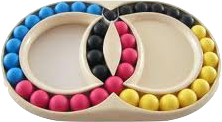
\includegraphics[width=1.0\linewidth,height=0.5\linewidth]{fig050001.png}
   \caption{"Hungarian Eight" \\ https://www.sfu.ca/~jtmulhol/math302/images/pic-puzzle-hr.png}
\label{fig050001}
\end{figure}

The game "Hungarian eight" (Fig. \ref{fig050001}) belongs to a group of logical puzzles, like the Rubik's cube. It consists of two intersecting circles, chutes filled with colored balls. The circles intersect at two points, so two balls belong to both chutes. The balls in the chutes can be rotated to scramble the puzzle. After the shuffle, the game's object is to arrange the marbles in the original state.

\section{Designing the Interface}

Although the game looks relatively simple, its arrangement involves relative complexity and quite a bit of mathematics. The organization of the puzzle itself is relatively simple, which makes it an ideal candidate for implementation in a programming environment such as Scratch. The entire game interface can be built with only thirty-eight dots and four arrows. Work begins with initiating a new project (Fig. \ref{fig050002}).

\begin{figure}[H]
   \centering
   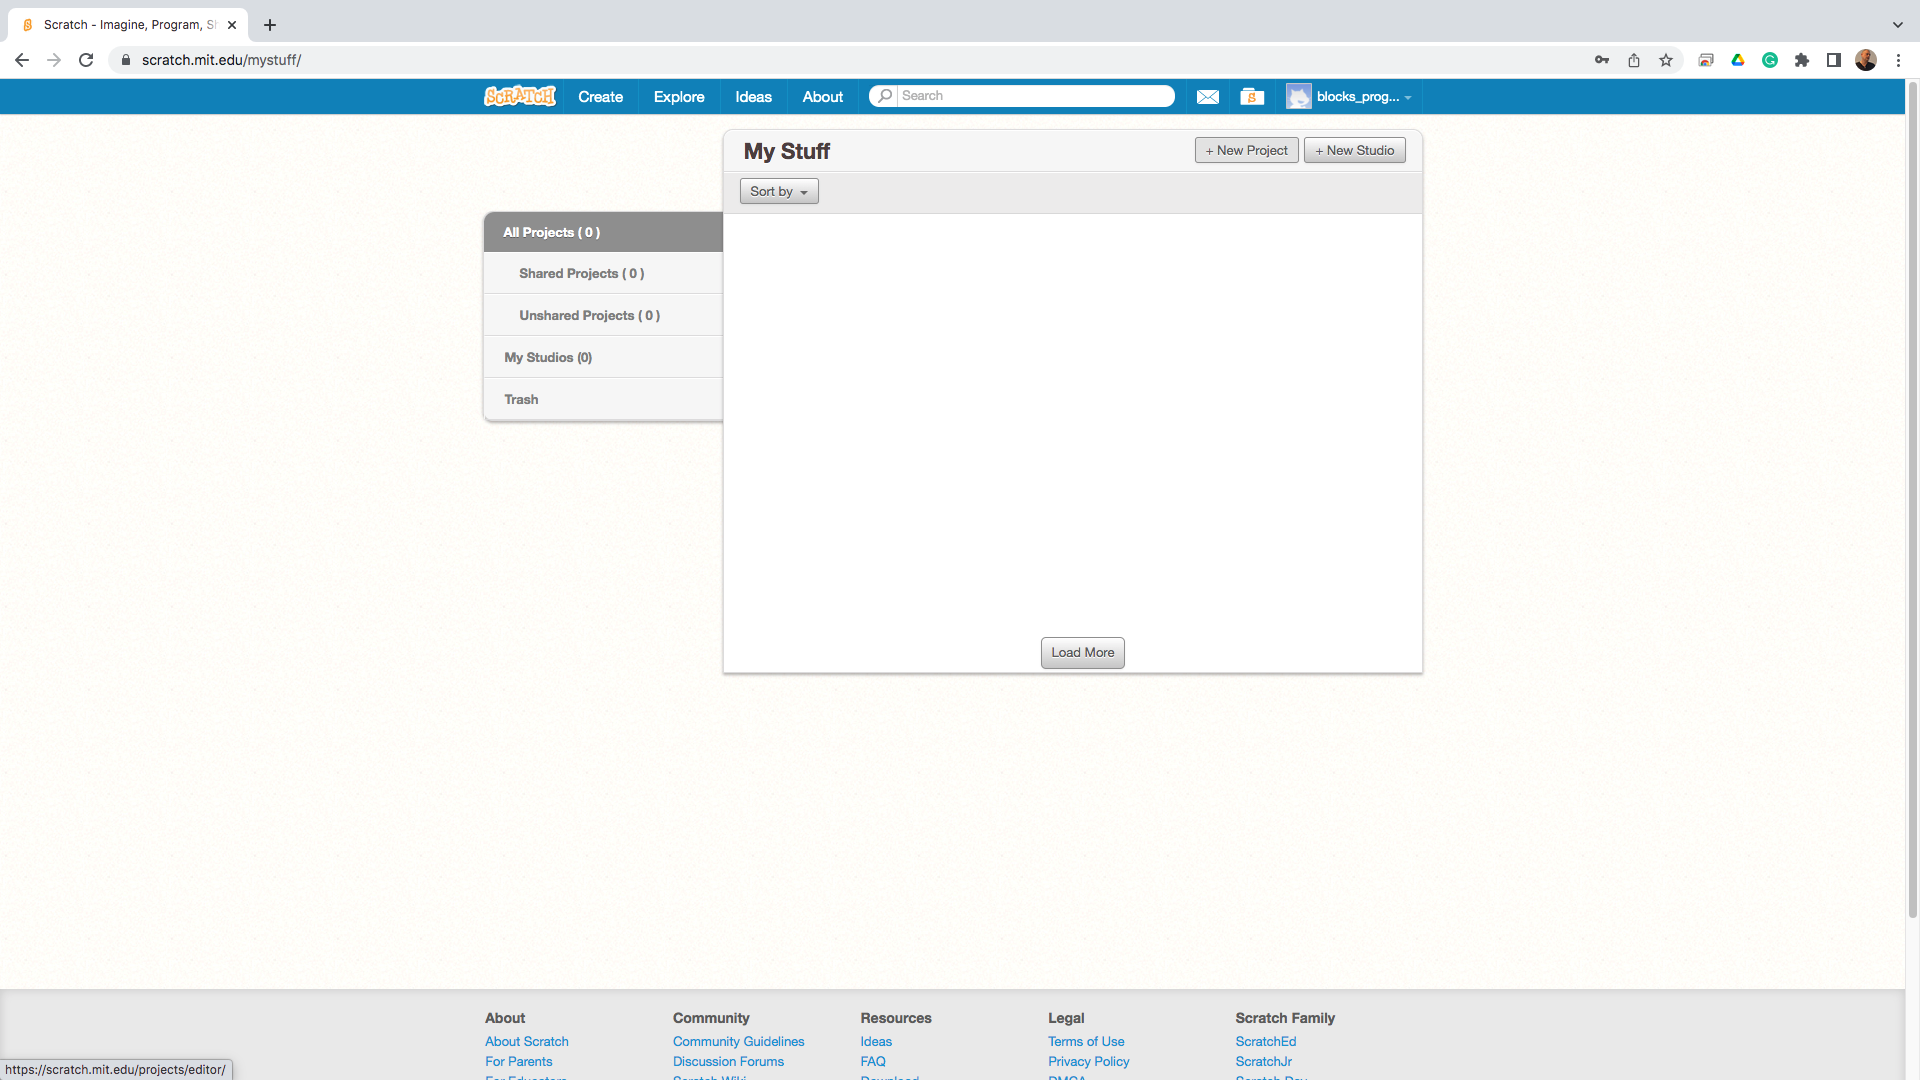
\includegraphics[width=1.0\linewidth,height=0.5\linewidth]{fig050002.png}
   \caption{Creating a "Hungarian Eight" project}
\label{fig050002}
\end{figure}

The first step is to choose a project name and accordingly clear the workspace of the cat sprite (Fig. \ref{fig050003}).

\begin{figure}[H]
   \centering
   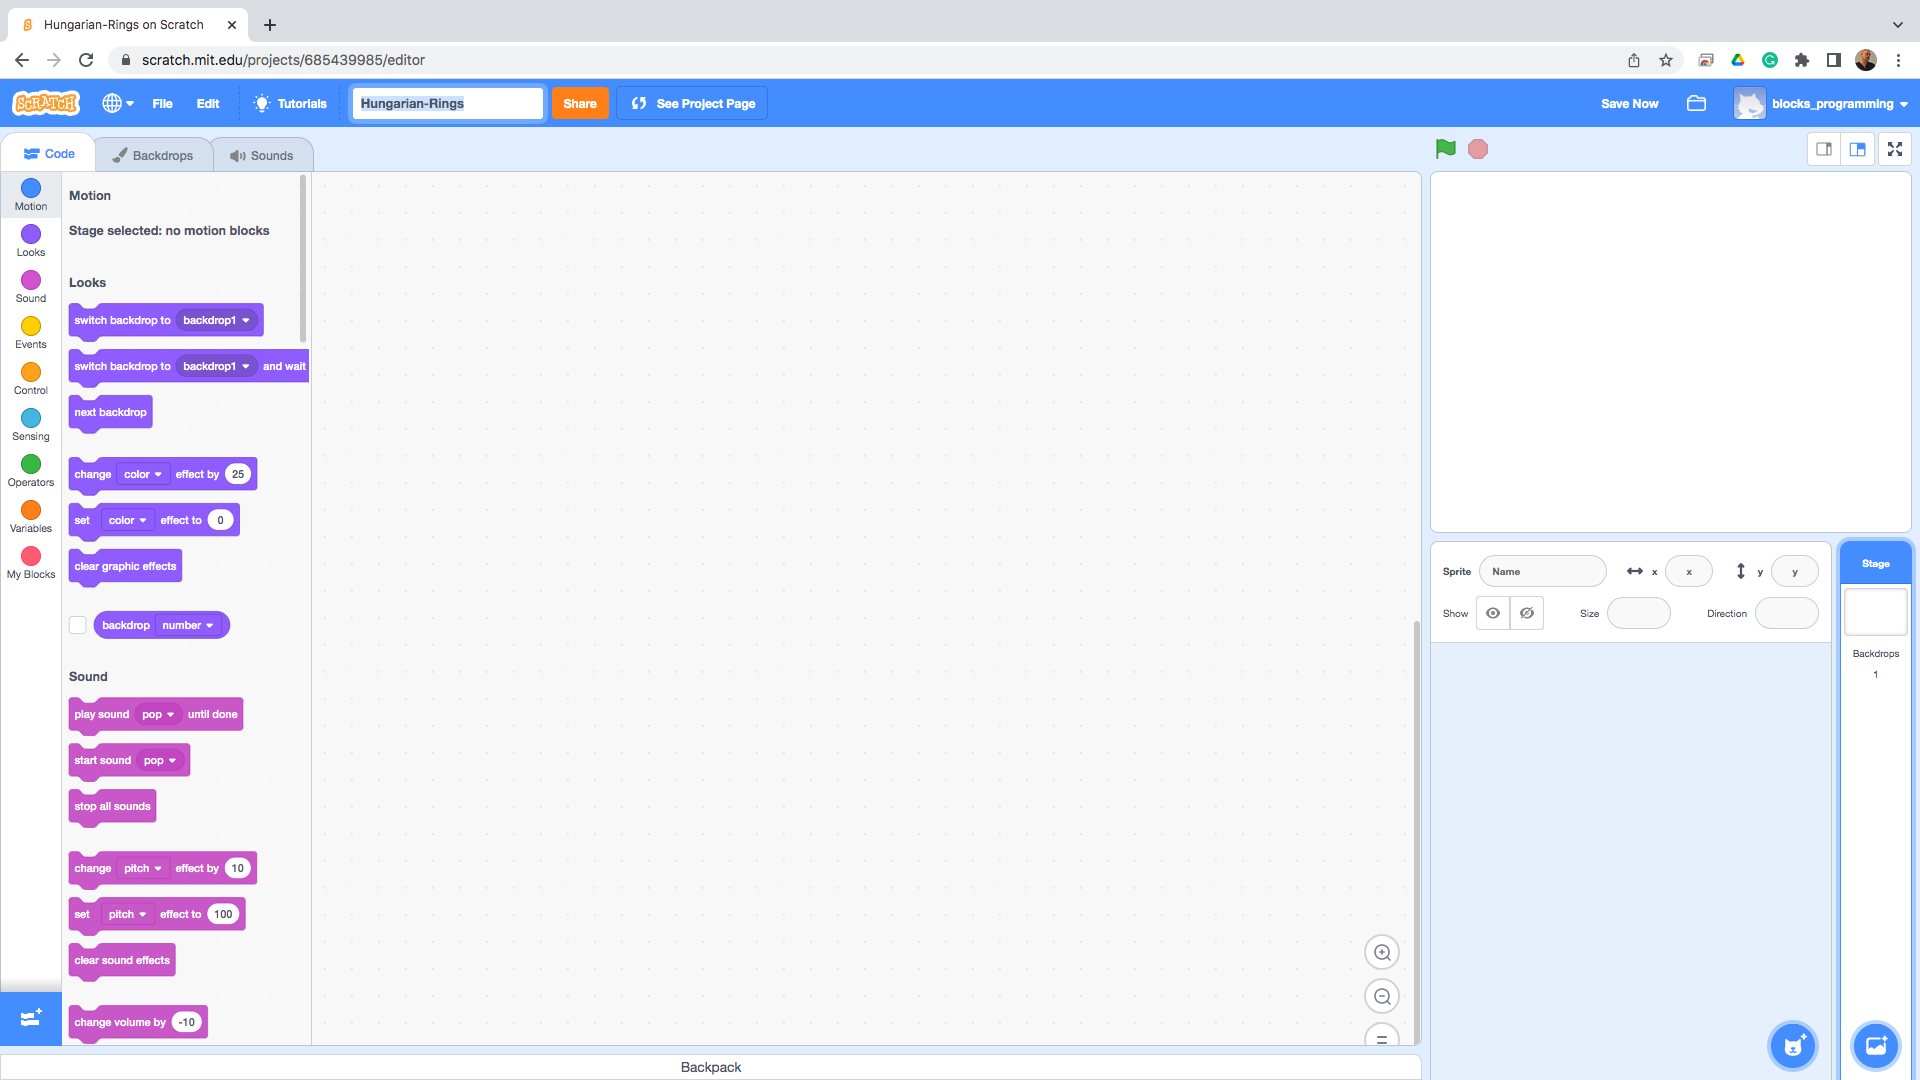
\includegraphics[width=1.0\linewidth,height=0.5\linewidth]{fig050003.png}
   \caption{Choose a name for the project}
\label{fig050003}
\end{figure}

Placing the colored balls (in this case, polka dots) is a relatively labor-intensive task, as two intersecting circles must be described. The work can be significantly facilitated if you work according to a previously prepared scheme (Fig. \ref{fig050004}). The polka dot pattern will only be visible until the rest of the sprites are lined up. In game mode, the scheme will be made invisible.

\begin{figure}[H]
   \centering
   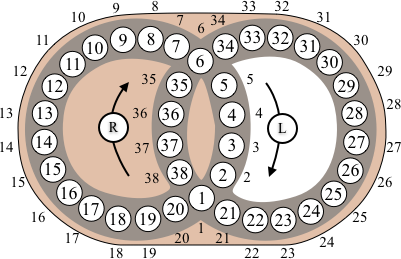
\includegraphics[width=1.0\linewidth,height=0.5\linewidth]{fig050004.png}
   \caption{Game diagram \\ https://www.sfu.ca/~jtmulhol/math302/images/hungarianrings-labeled-nocolor.png}
\label{fig050004}
\end{figure}

The graphics file for the game layout is added to the sprite group using the add icon (Fig. \ref{fig050005}).

\begin{figure}[H]
   \centering
   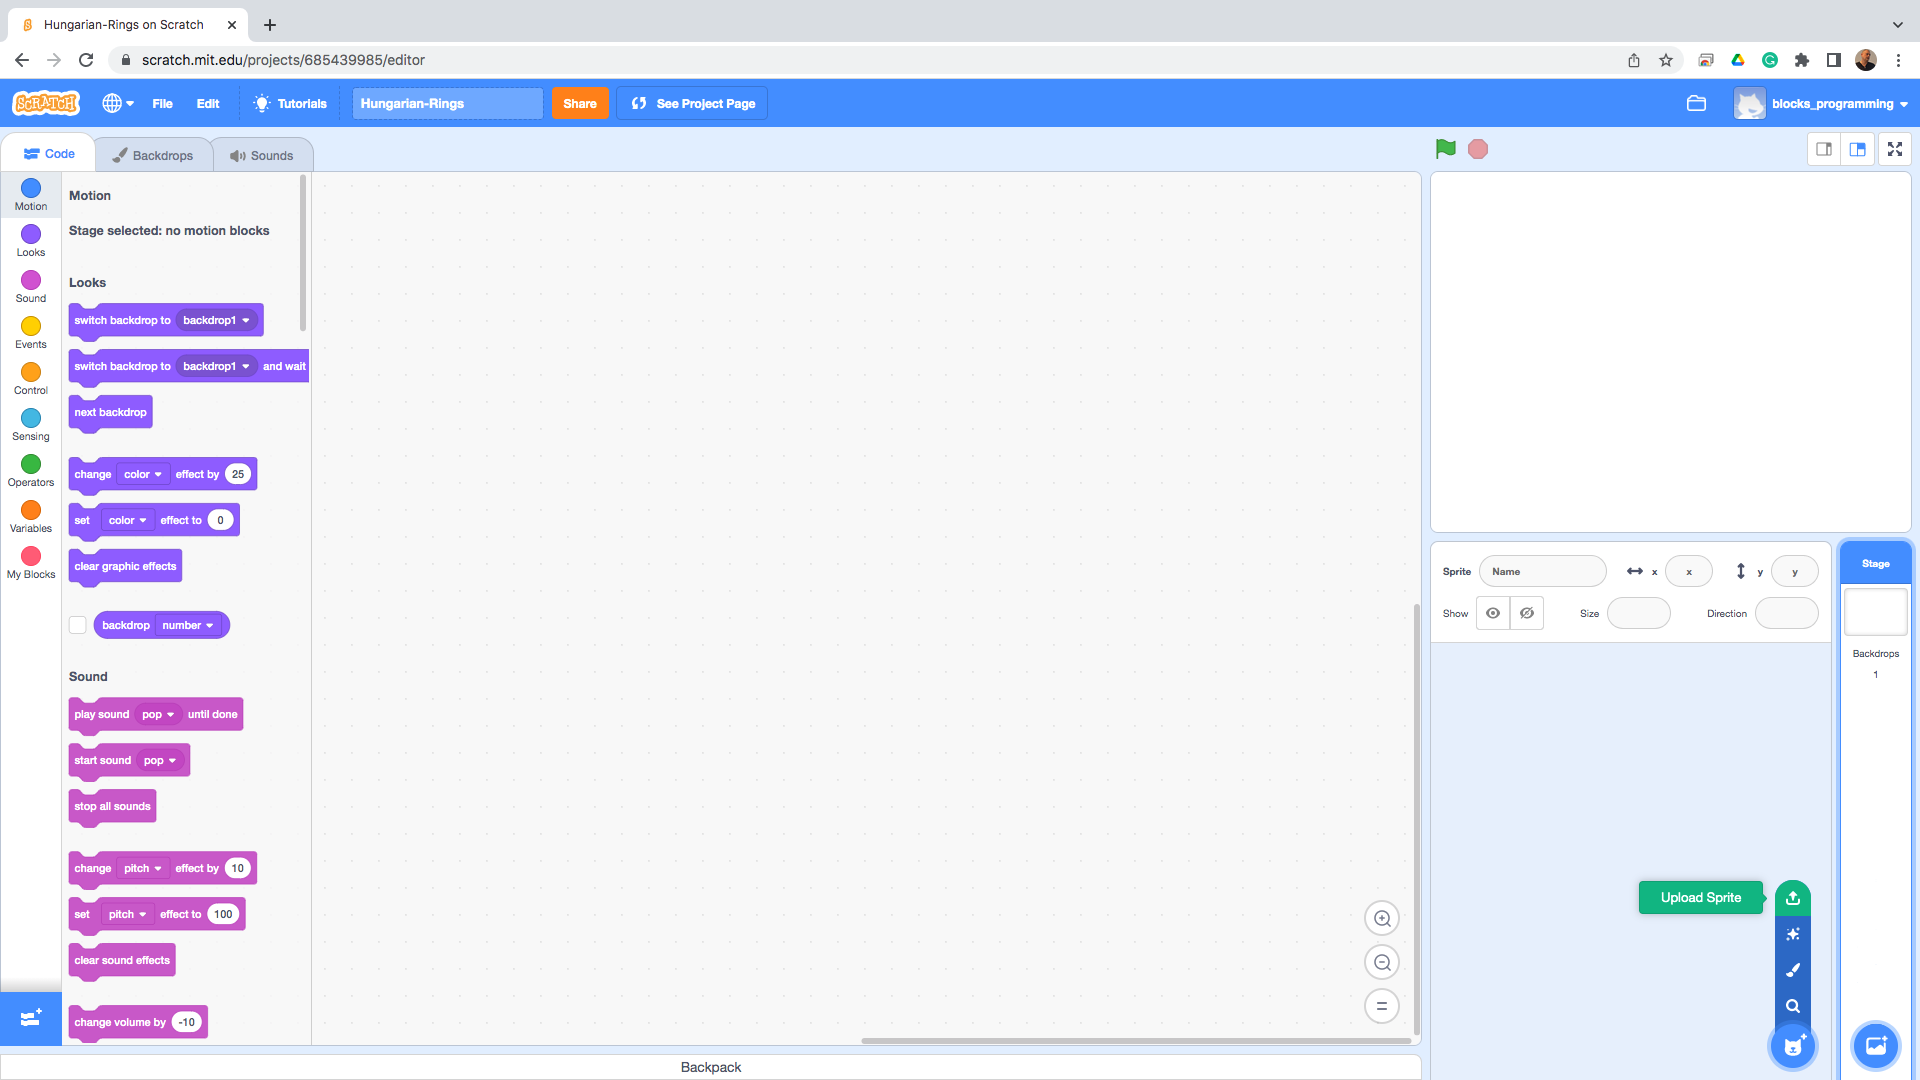
\includegraphics[width=1.0\linewidth,height=0.5\linewidth]{fig050005.png}
   \caption{Add the image for the game outline}
\label{fig050005}
\end{figure}

The newly added sprite is centered at coordinates x=0 and y=0 (Fig. \ref{fig050006}) to achieve visual symmetry, and the images of the balls to be added are in the middle of the visual space.

\begin{figure}[H]
   \centering
   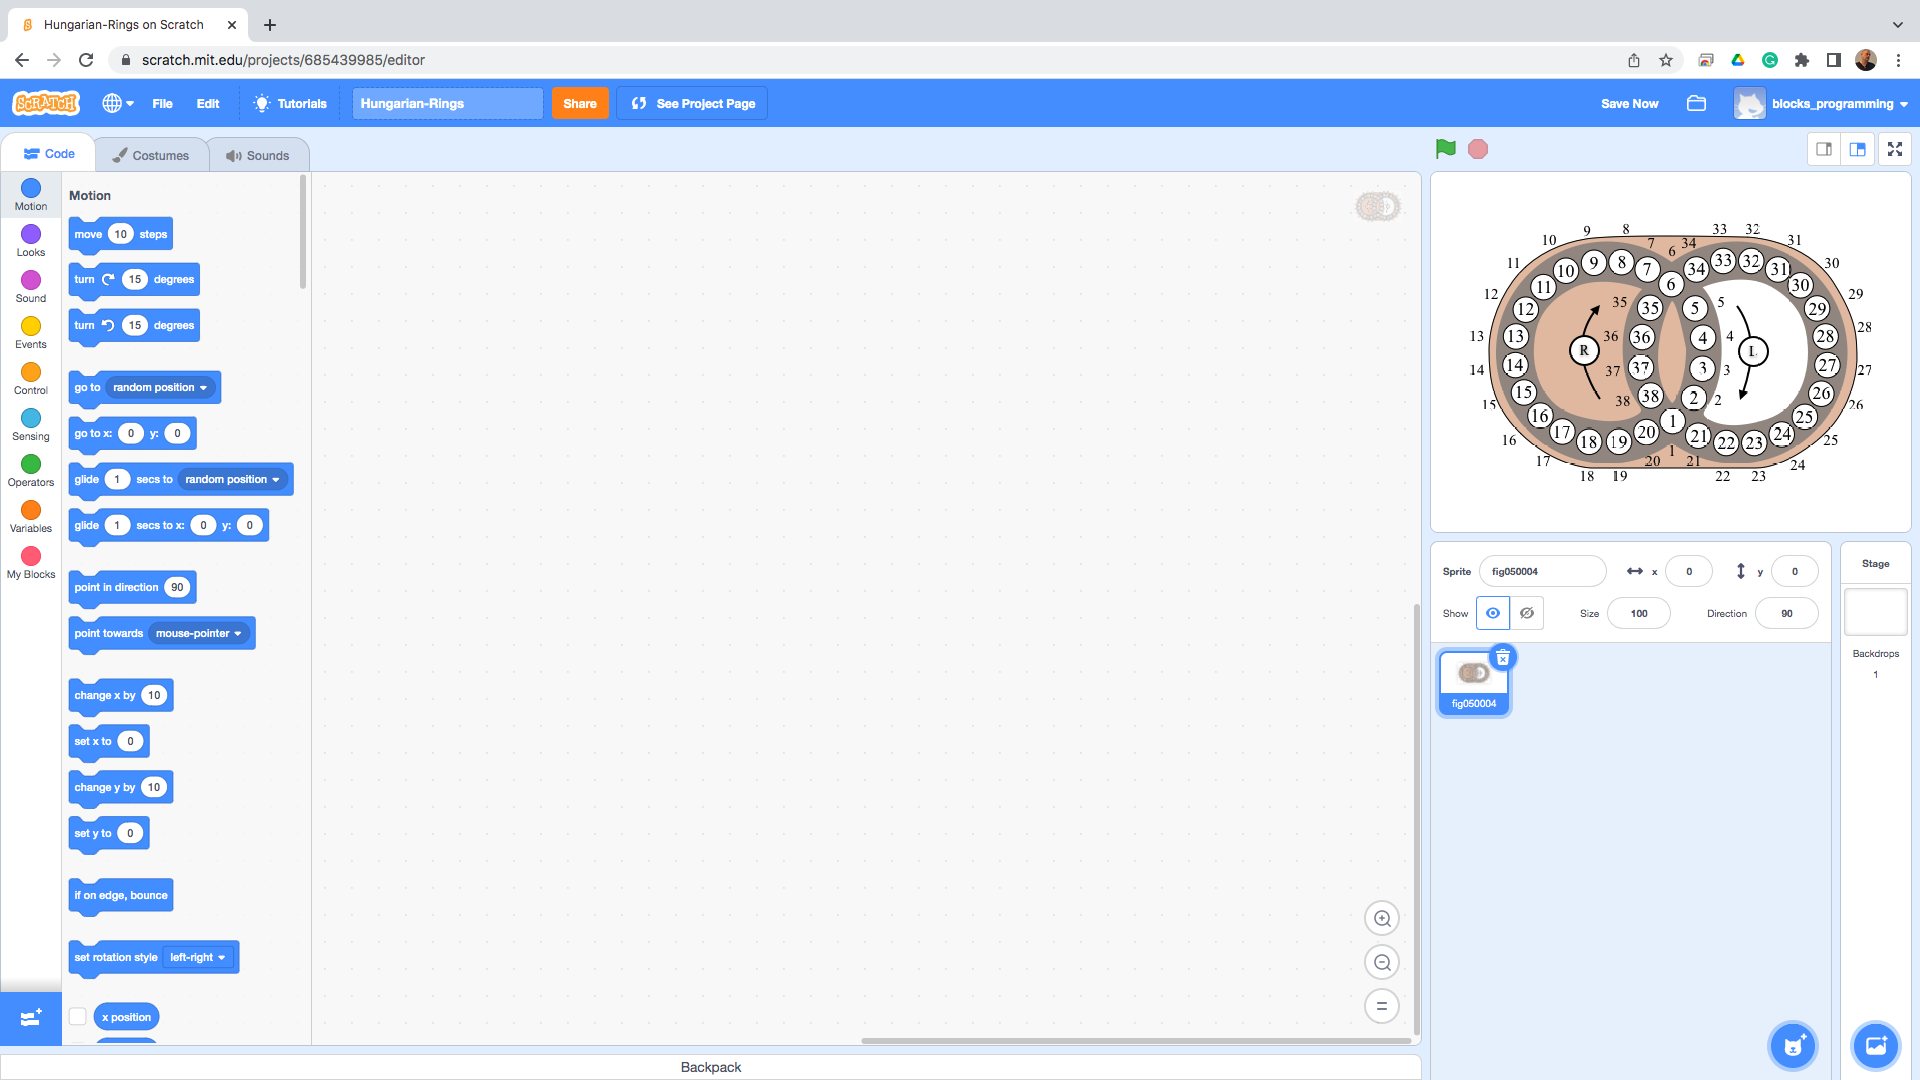
\includegraphics[width=1.0\linewidth,height=0.5\linewidth]{fig050006.png}
   \caption{Center the diagram}
\label{fig050006}
\end{figure}

From the gallery of pre-available sprites (Fig. \ref{fig050007}), you can choose a suitable sprite for the arrows that will cause the rotation of the two circles.

\begin{figure}[H]
   \centering
   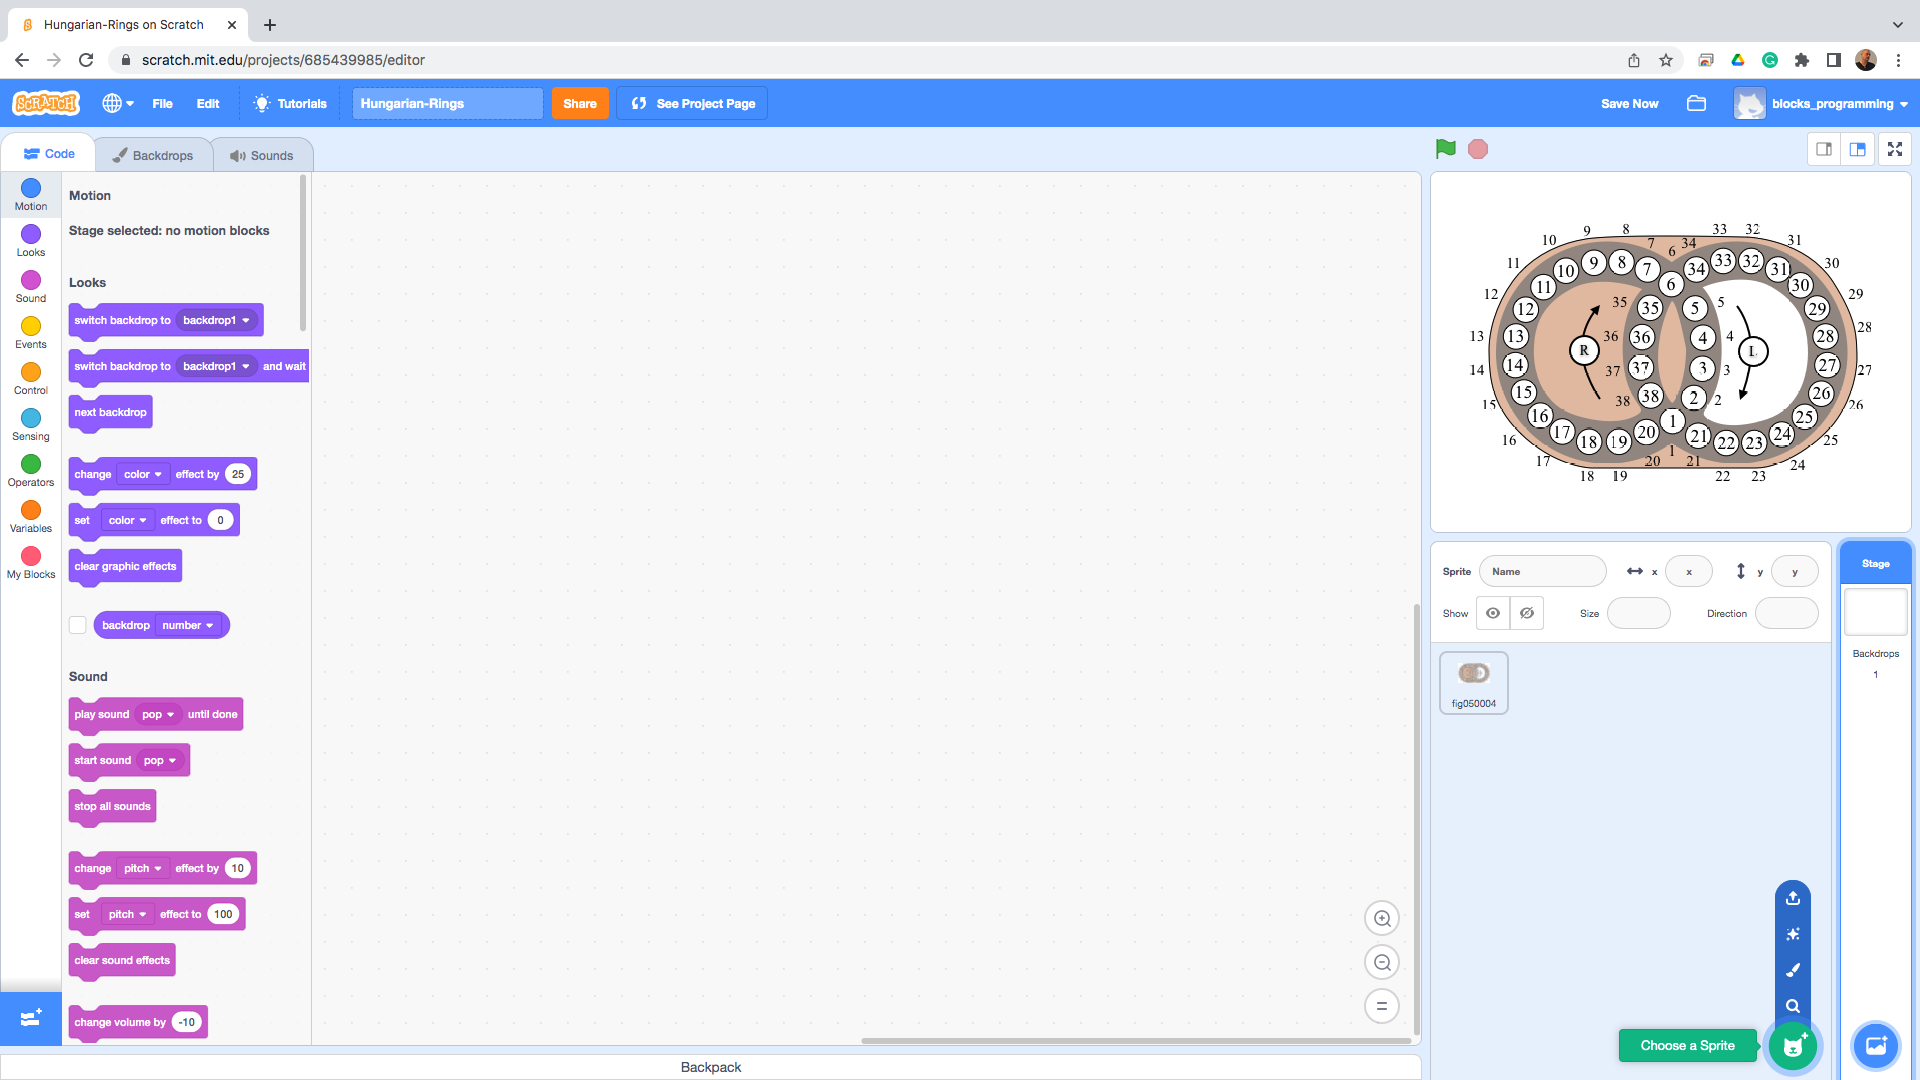
\includegraphics[width=1.0\linewidth,height=0.5\linewidth]{fig050007.png}
   \caption{Gallery of pre-available sprites}
\label{fig050007}
\end{figure}

The arrow sprite has four states (Fig. \ref{fig050008}) that allow this sprite to be used for rotation directions.

\begin{figure}[H]
   \centering
   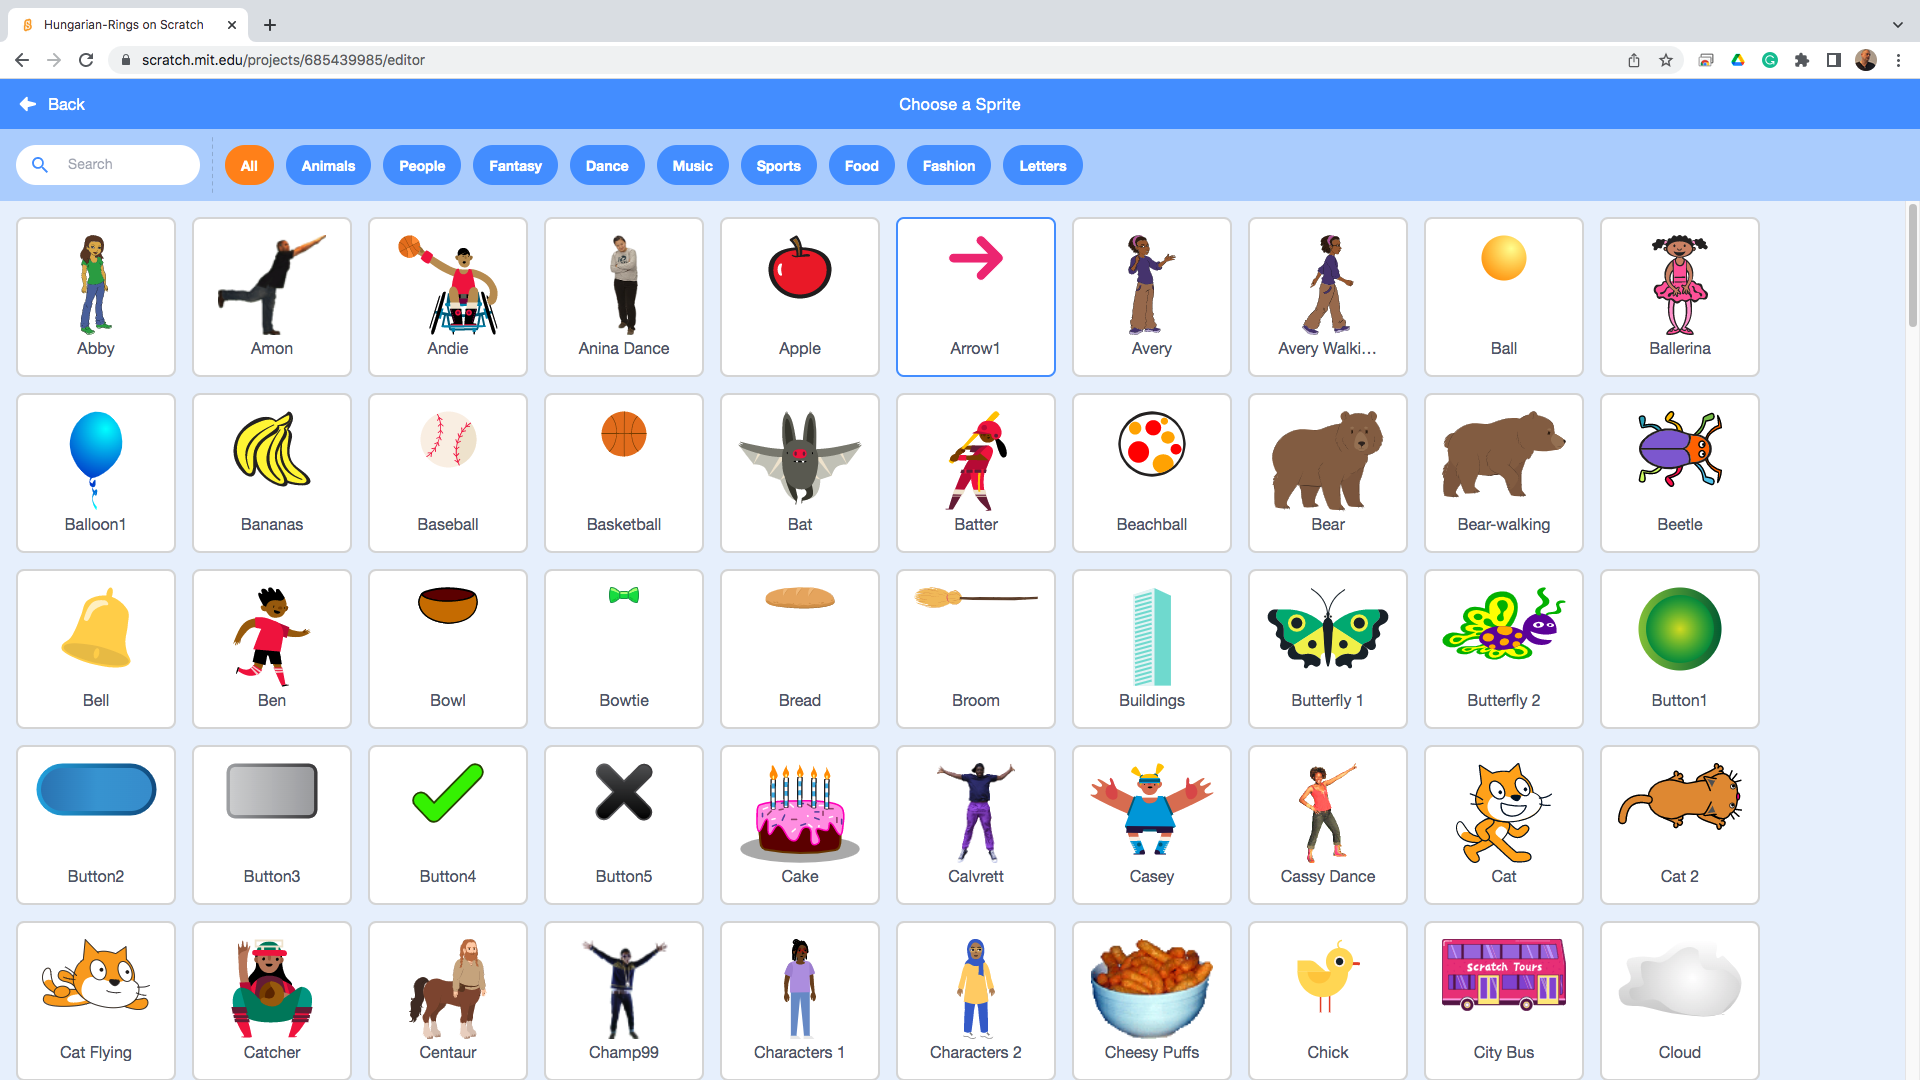
\includegraphics[width=1.0\linewidth,height=0.5\linewidth]{fig050008.png}
   \caption{Arrow Sprite}
\label{fig050008}
\end{figure}

The first arrow is located at the top right (Fig. \ref{fig050009}) and will rotate the right ring clockwise.

\begin{figure}[H]
   \centering
   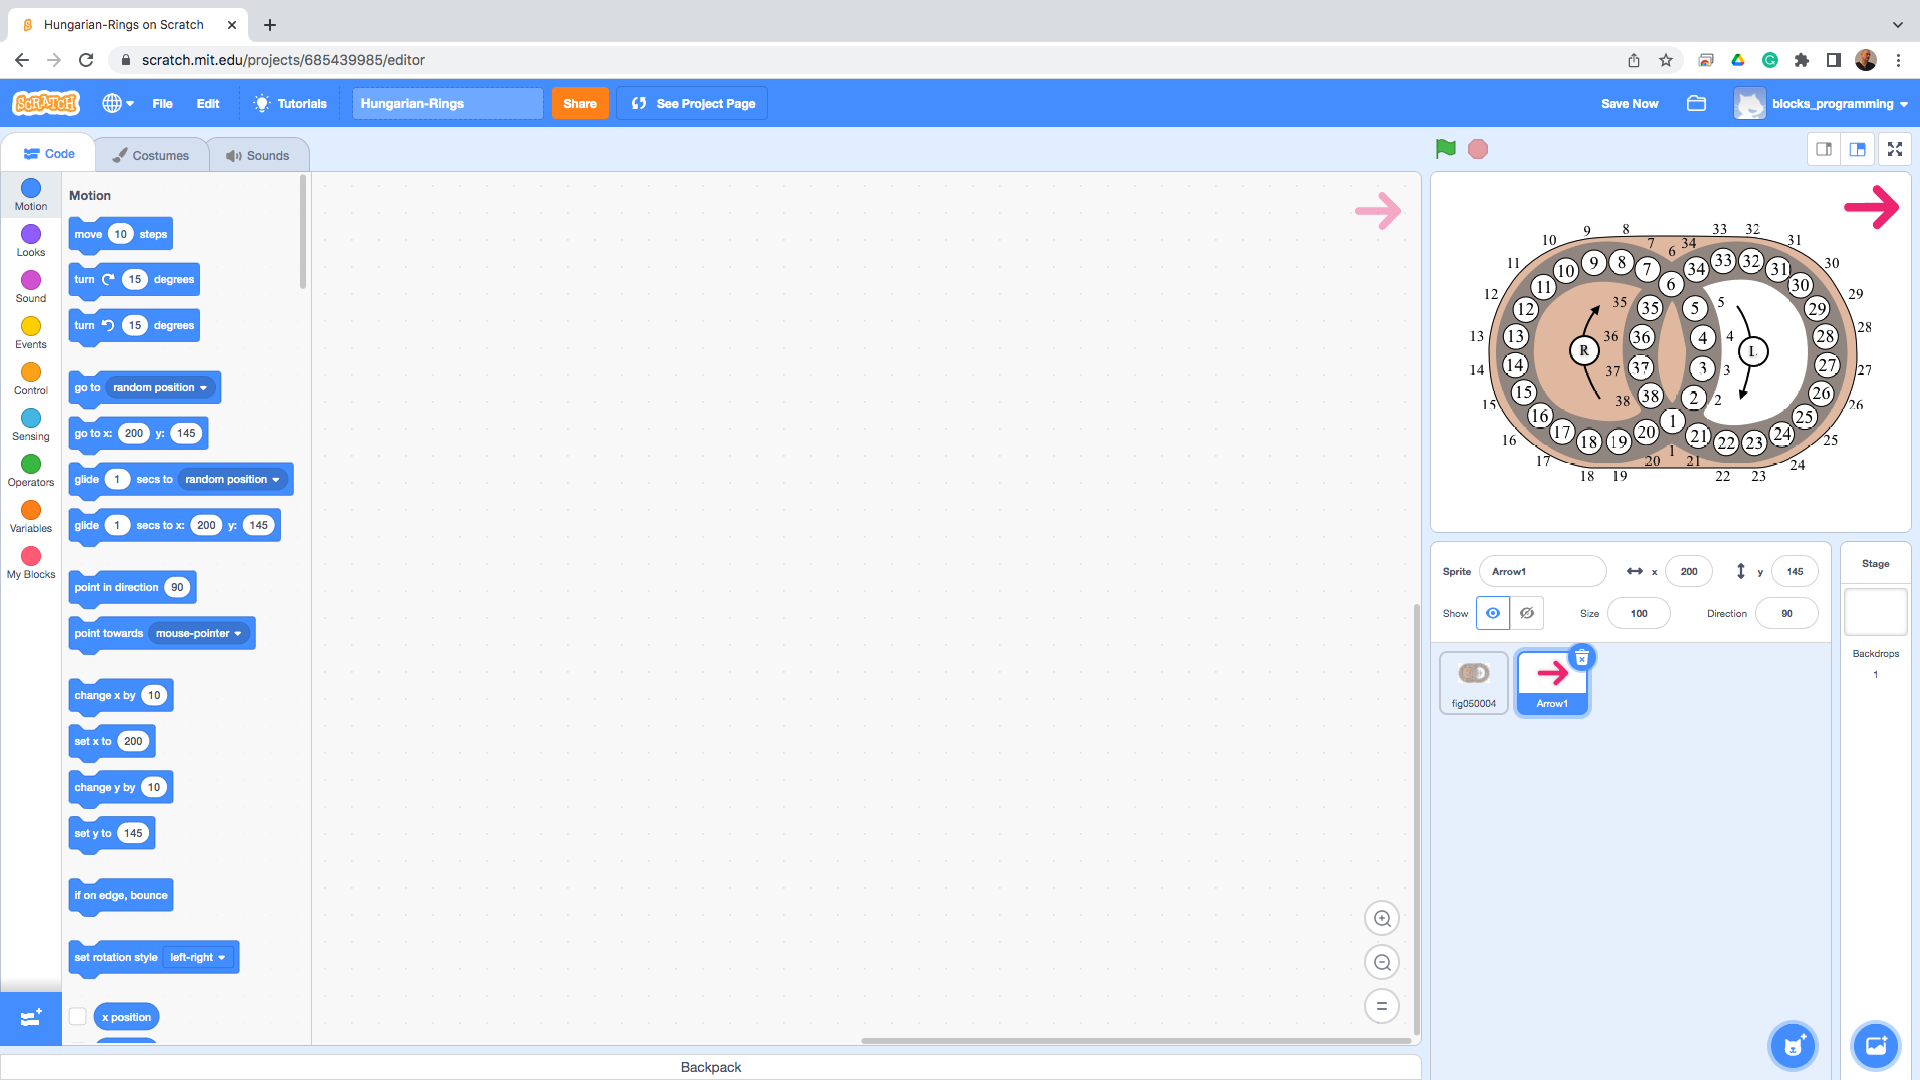
\includegraphics[width=1.0\linewidth,height=0.5\linewidth]{fig050009.png}
   \caption{Arrow to rotate right ring clockwise}
\label{fig050009}
\end{figure}

The second arrow is located at the bottom right (Fig. \ref{fig050010}) and will rotate the right ring counter-clockwise.

\begin{figure}[H]
   \centering
   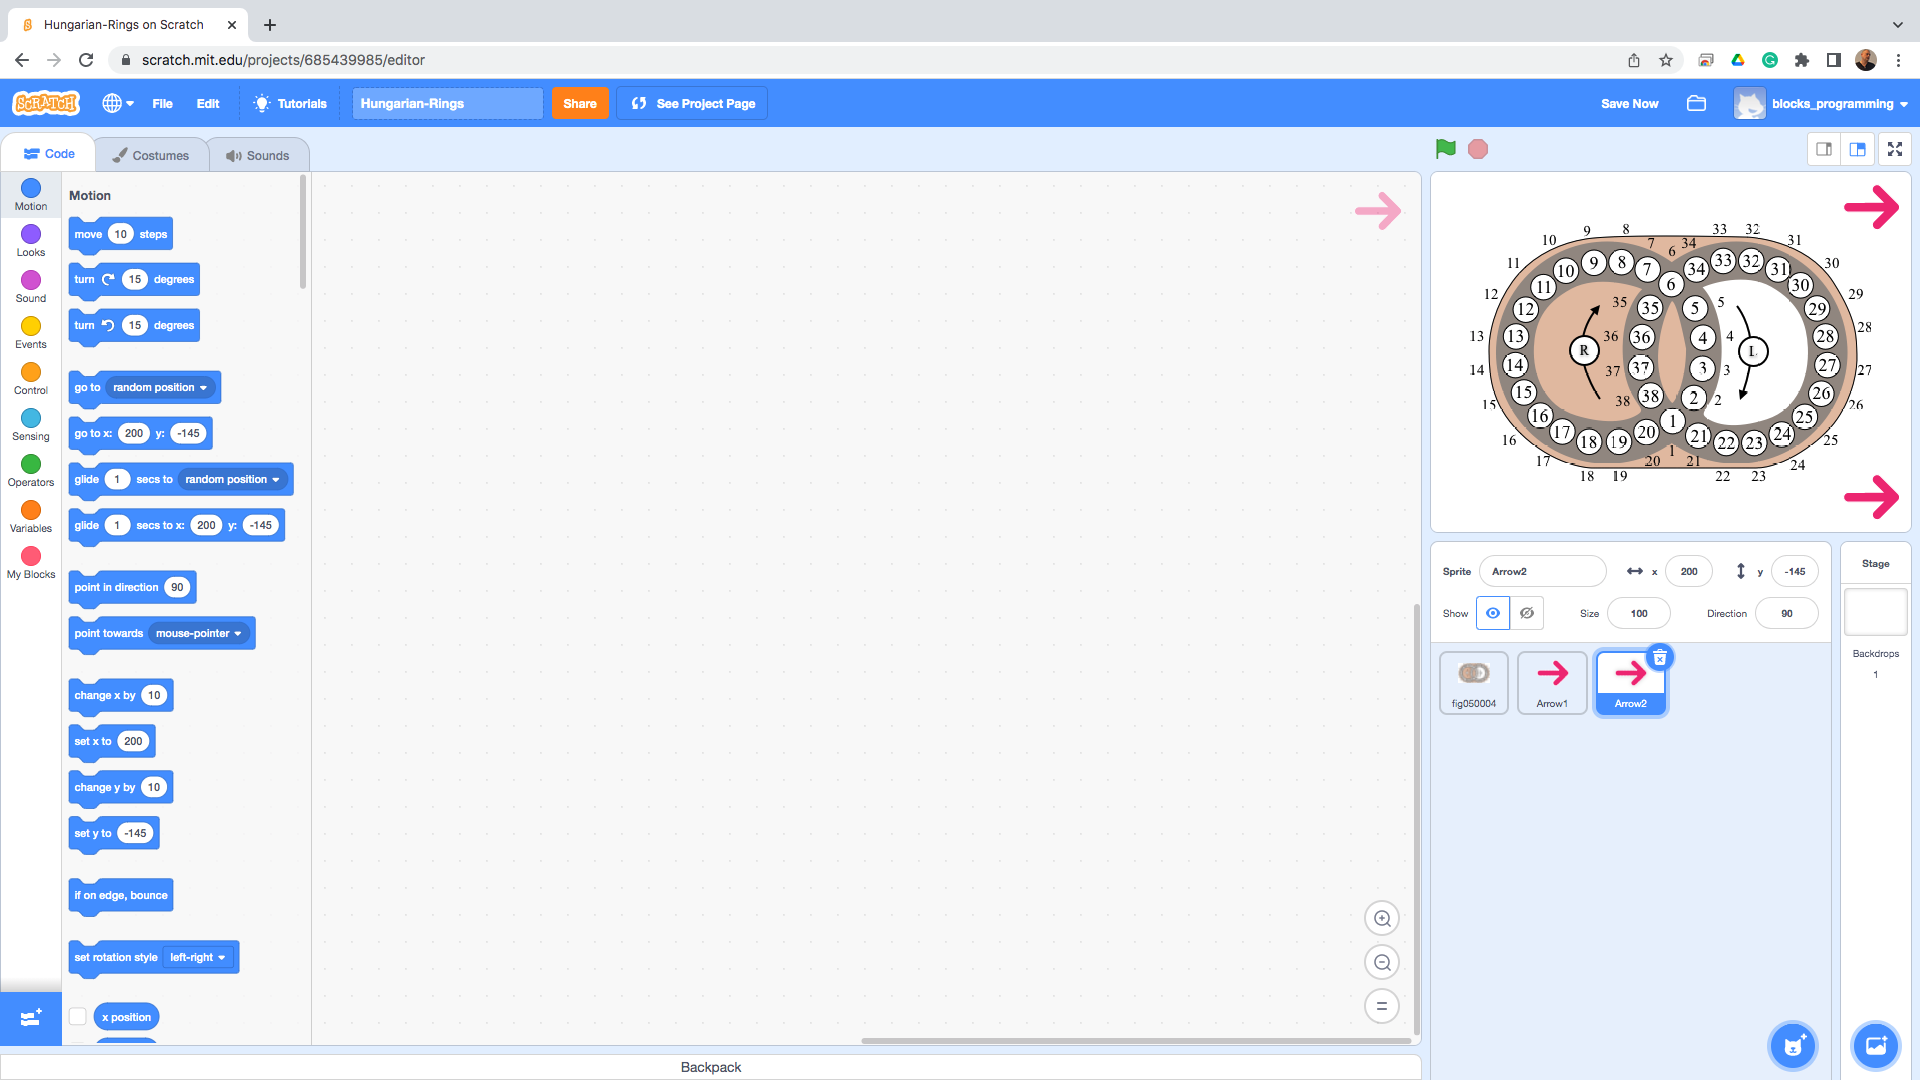
\includegraphics[width=1.0\linewidth,height=0.5\linewidth]{fig050010.png}
   \caption{Arrow to rotate right ring counterclockwise}
\label{fig050010}
\end{figure}

The third arrow is positioned at the bottom-left by selecting the second frame in the sprite as active so that the arrow points to the left (Fig. \ref{fig050011}).

\begin{figure}[H]
   \centering
   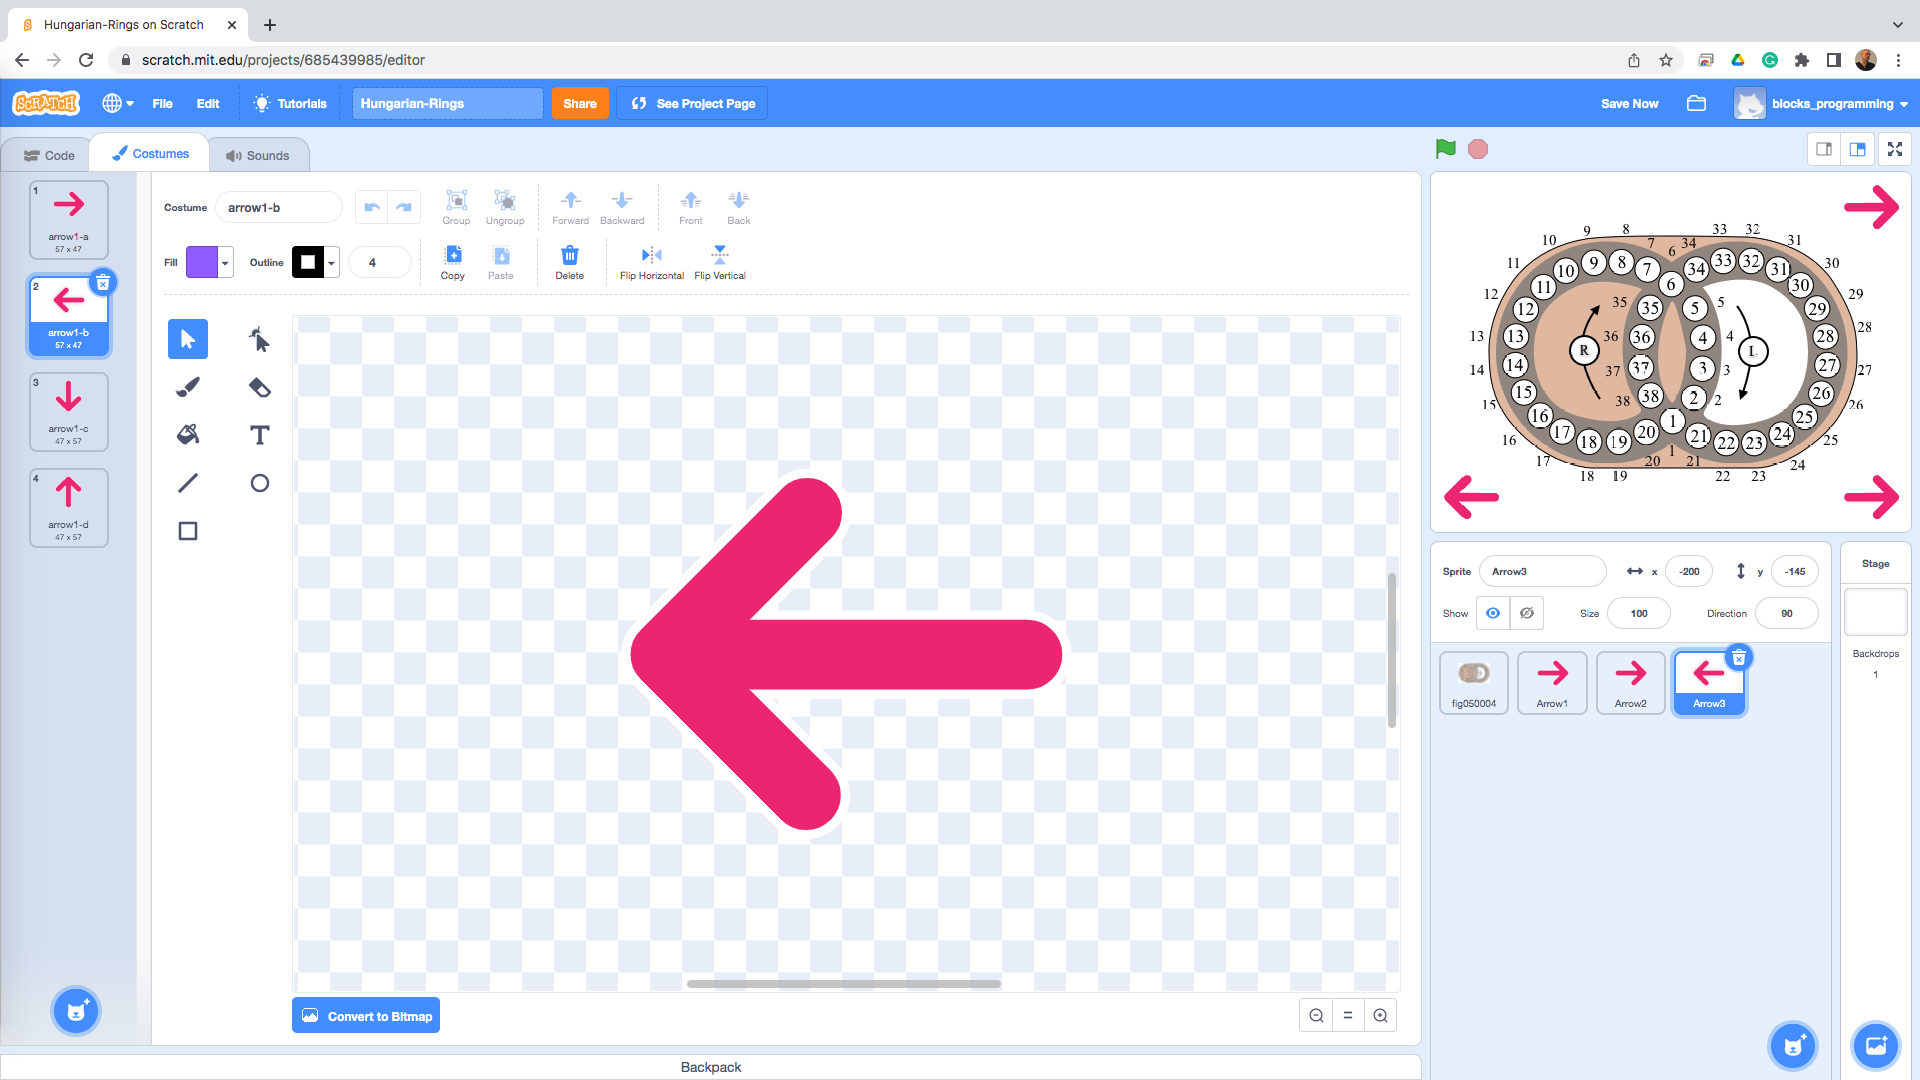
\includegraphics[width=1.0\linewidth,height=0.5\linewidth]{fig050011.png}
   \caption{Left ring clockwise rotation arrow}
\label{fig050011}
\end{figure}

The fourth arrow is located at the top-left (Fig. \ref{fig050012}), and its task is to cause the left ring to rotate in the counterclockwise direction.

\begin{figure}[H]
   \centering
   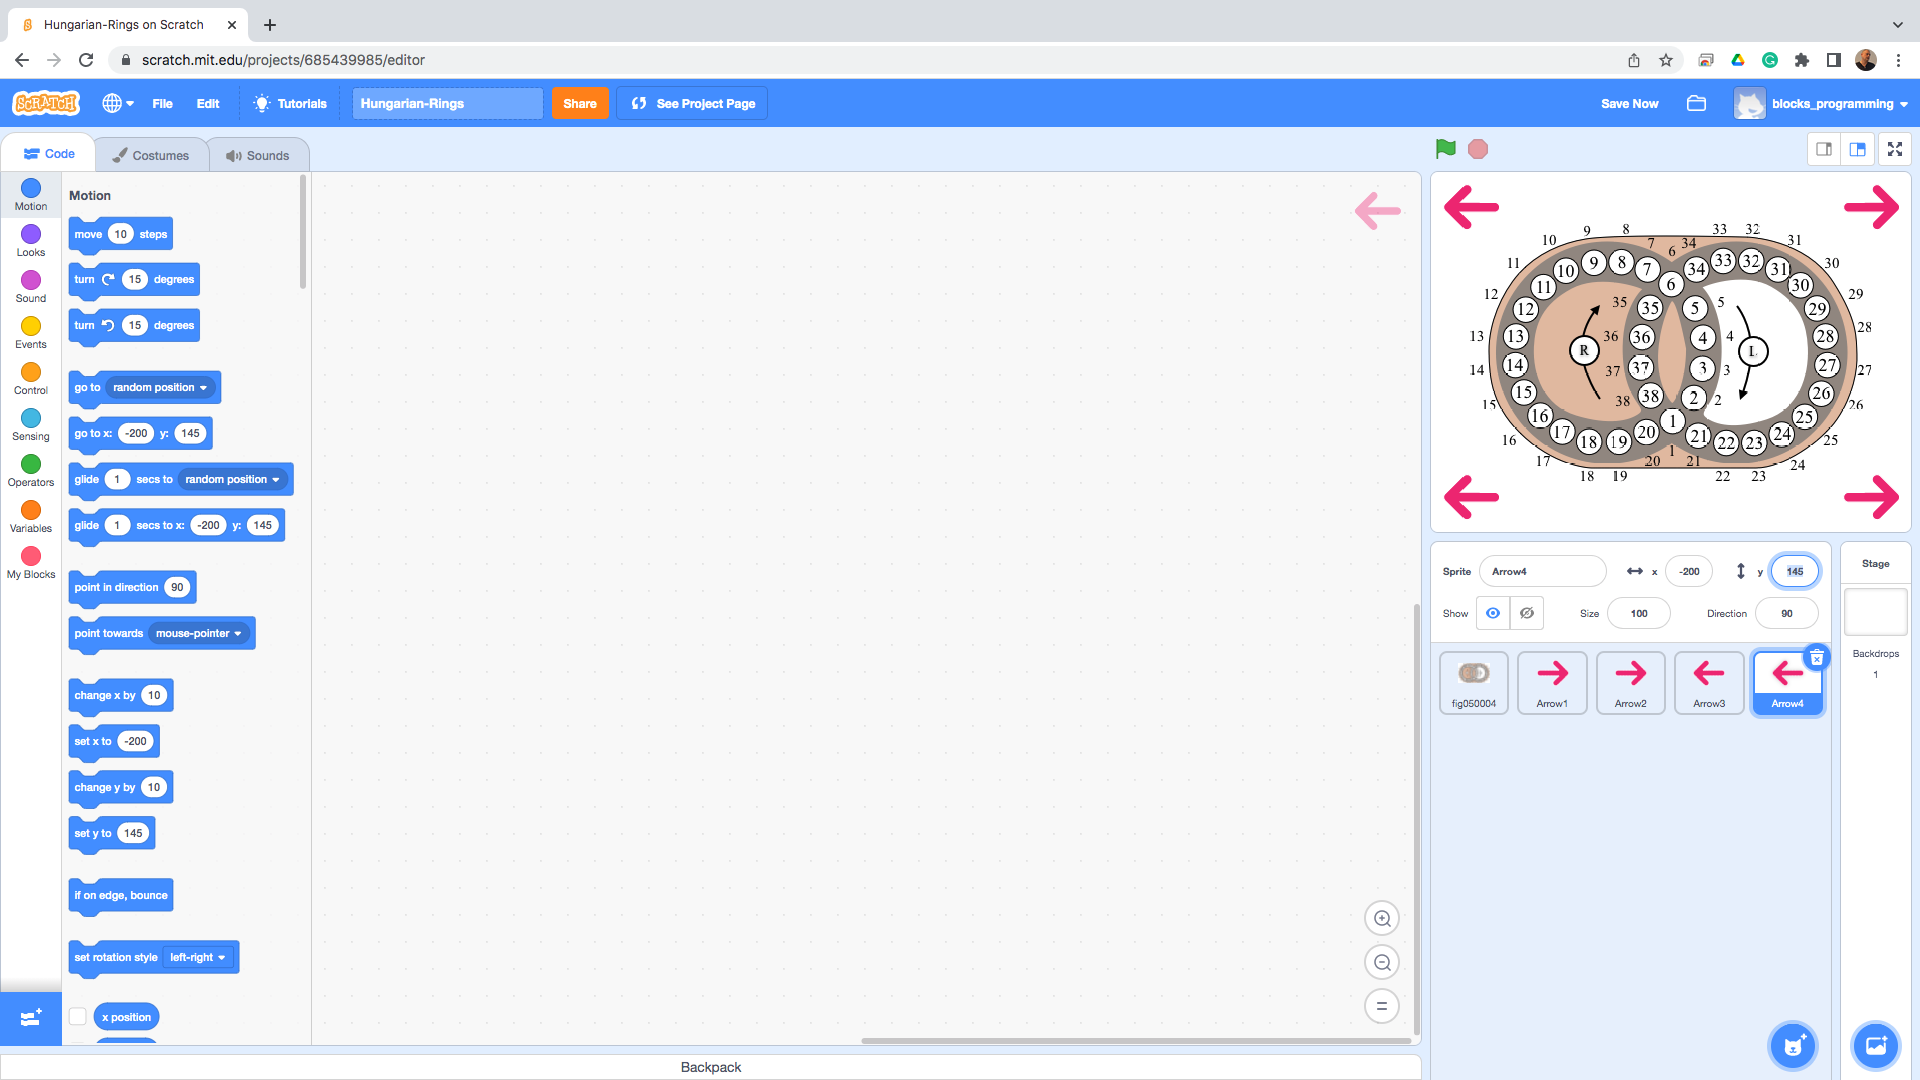
\includegraphics[width=1.0\linewidth,height=0.5\linewidth]{fig050012.png}
   \caption{Left ring counter-clockwise rotation arrow}
\label{fig050012}
\end{figure}

One way to visualize the balls from the original game is through a ball sprite (Fig. \ref{fig050013}). This sprite allows the ball to be rendered in several colors, perfectly fitting the need to render four different colored balls.

\begin{figure}[H]
   \centering
   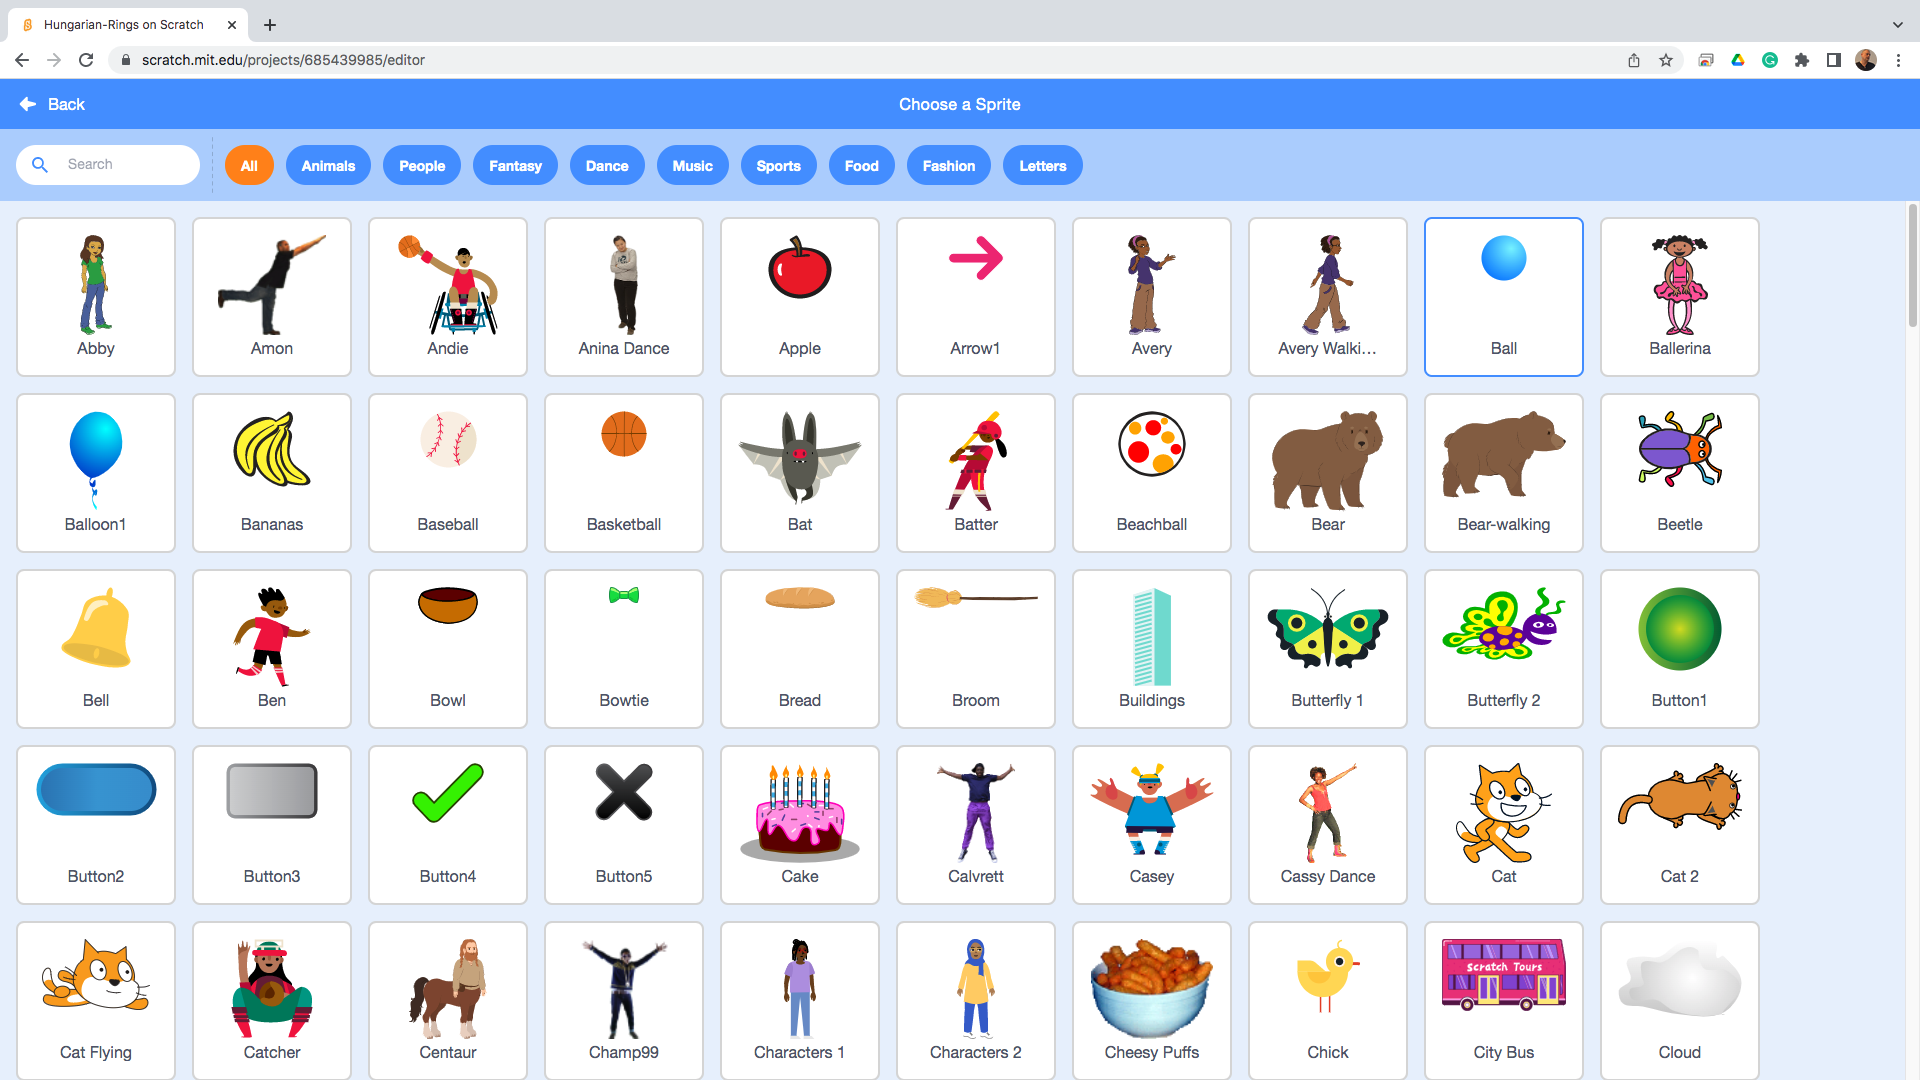
\includegraphics[width=1.0\linewidth,height=0.5\linewidth]{fig050013.png}
   \caption{Choosing a sprite for the points}
\label{fig050013}
\end{figure}

The first checker placed goes to the position marked with the number one on the already included pattern. To successfully overlay the different sprites, it is necessary to send the schematic sprite to the back of the Z-buffer so that all other sprites are rendered in front of it.

The ball is shrunk (in this case to 55) and then adjusted with the mouse to fit precisely on the space marked with a unit (Fig. \ref{fig050014}).

\begin{figure}[H]
   \centering
   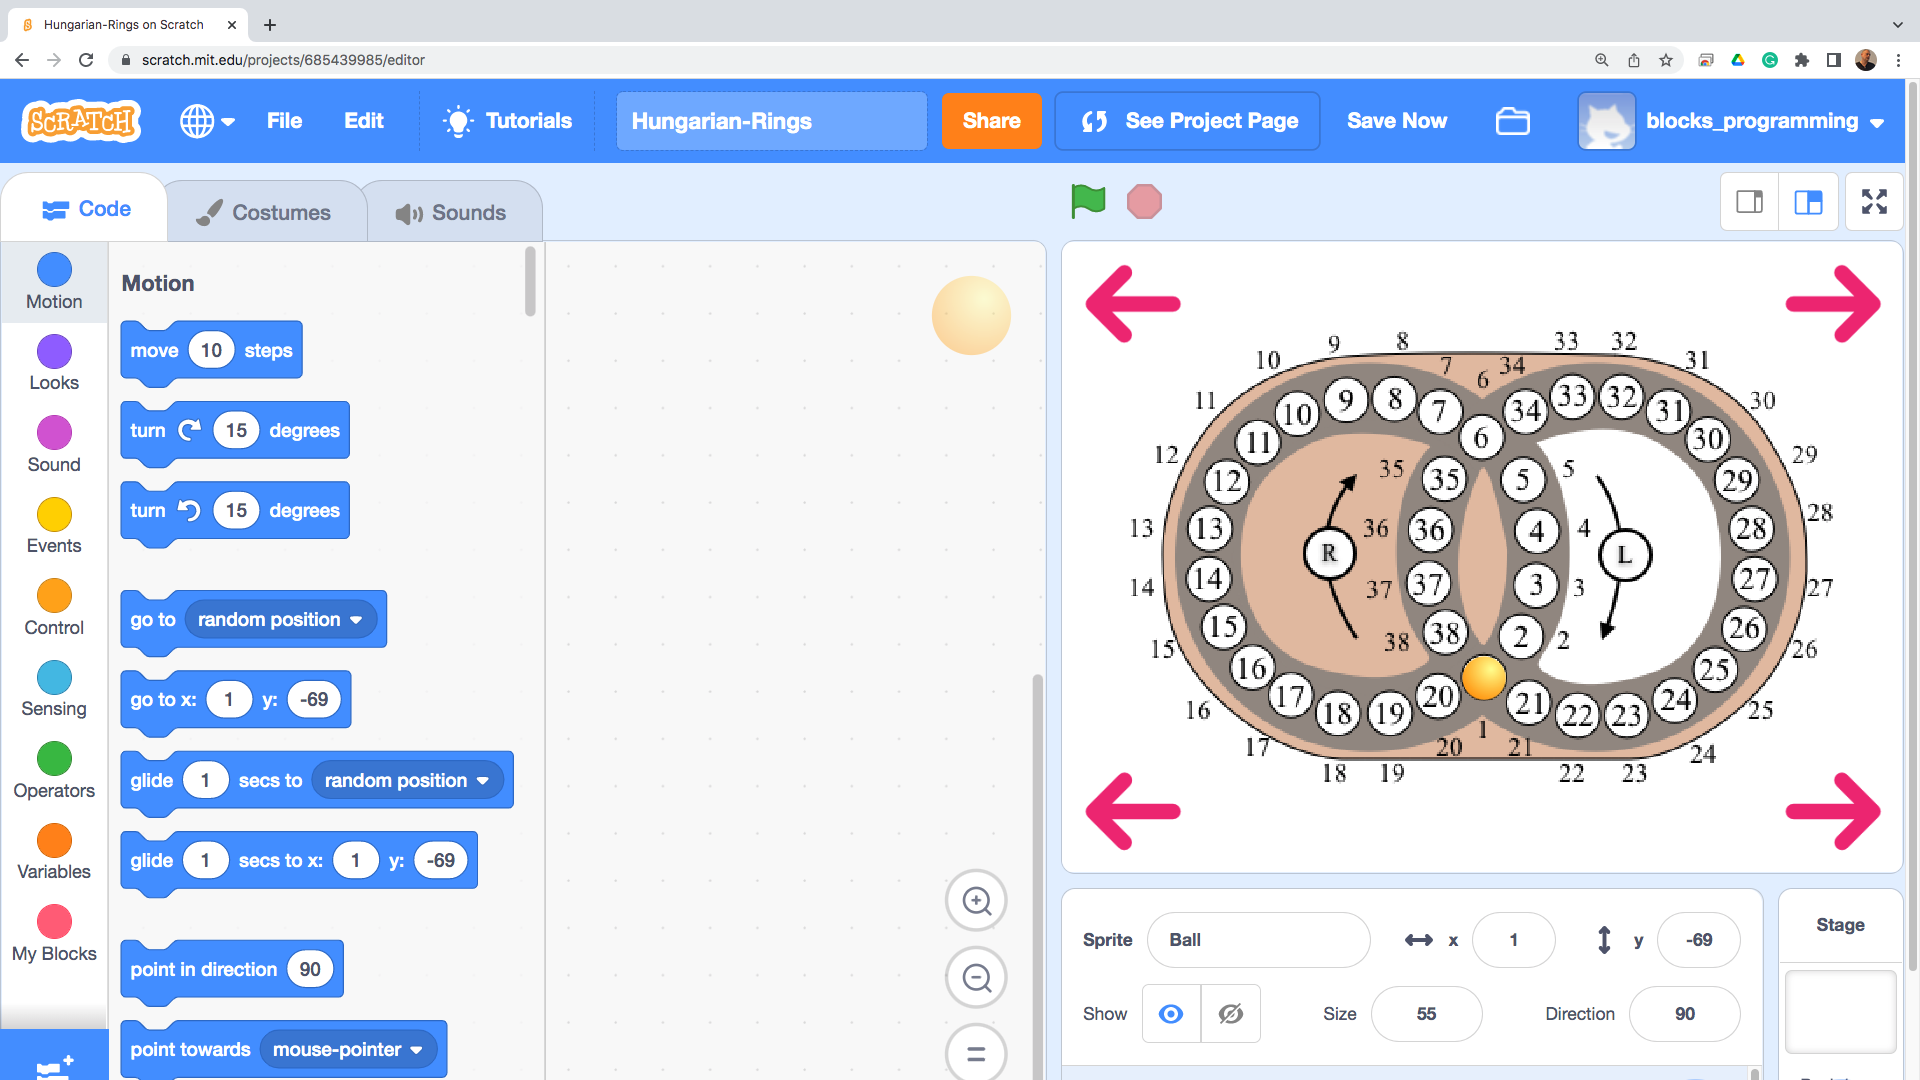
\includegraphics[width=1.0\linewidth,height=0.5\linewidth]{fig050014.png}
   \caption{Sizing and positioning the first bead}
\label{fig050014}
\end{figure}

\section{Data Structures}

When the yoke starts (Fig. \ref{fig050015}), the state of the playing field will be reflected in a list structure. The numbers one through four will reflect what color ball should be visualized in the corresponding numbered position.

\begin{figure}[H]
   \centering
   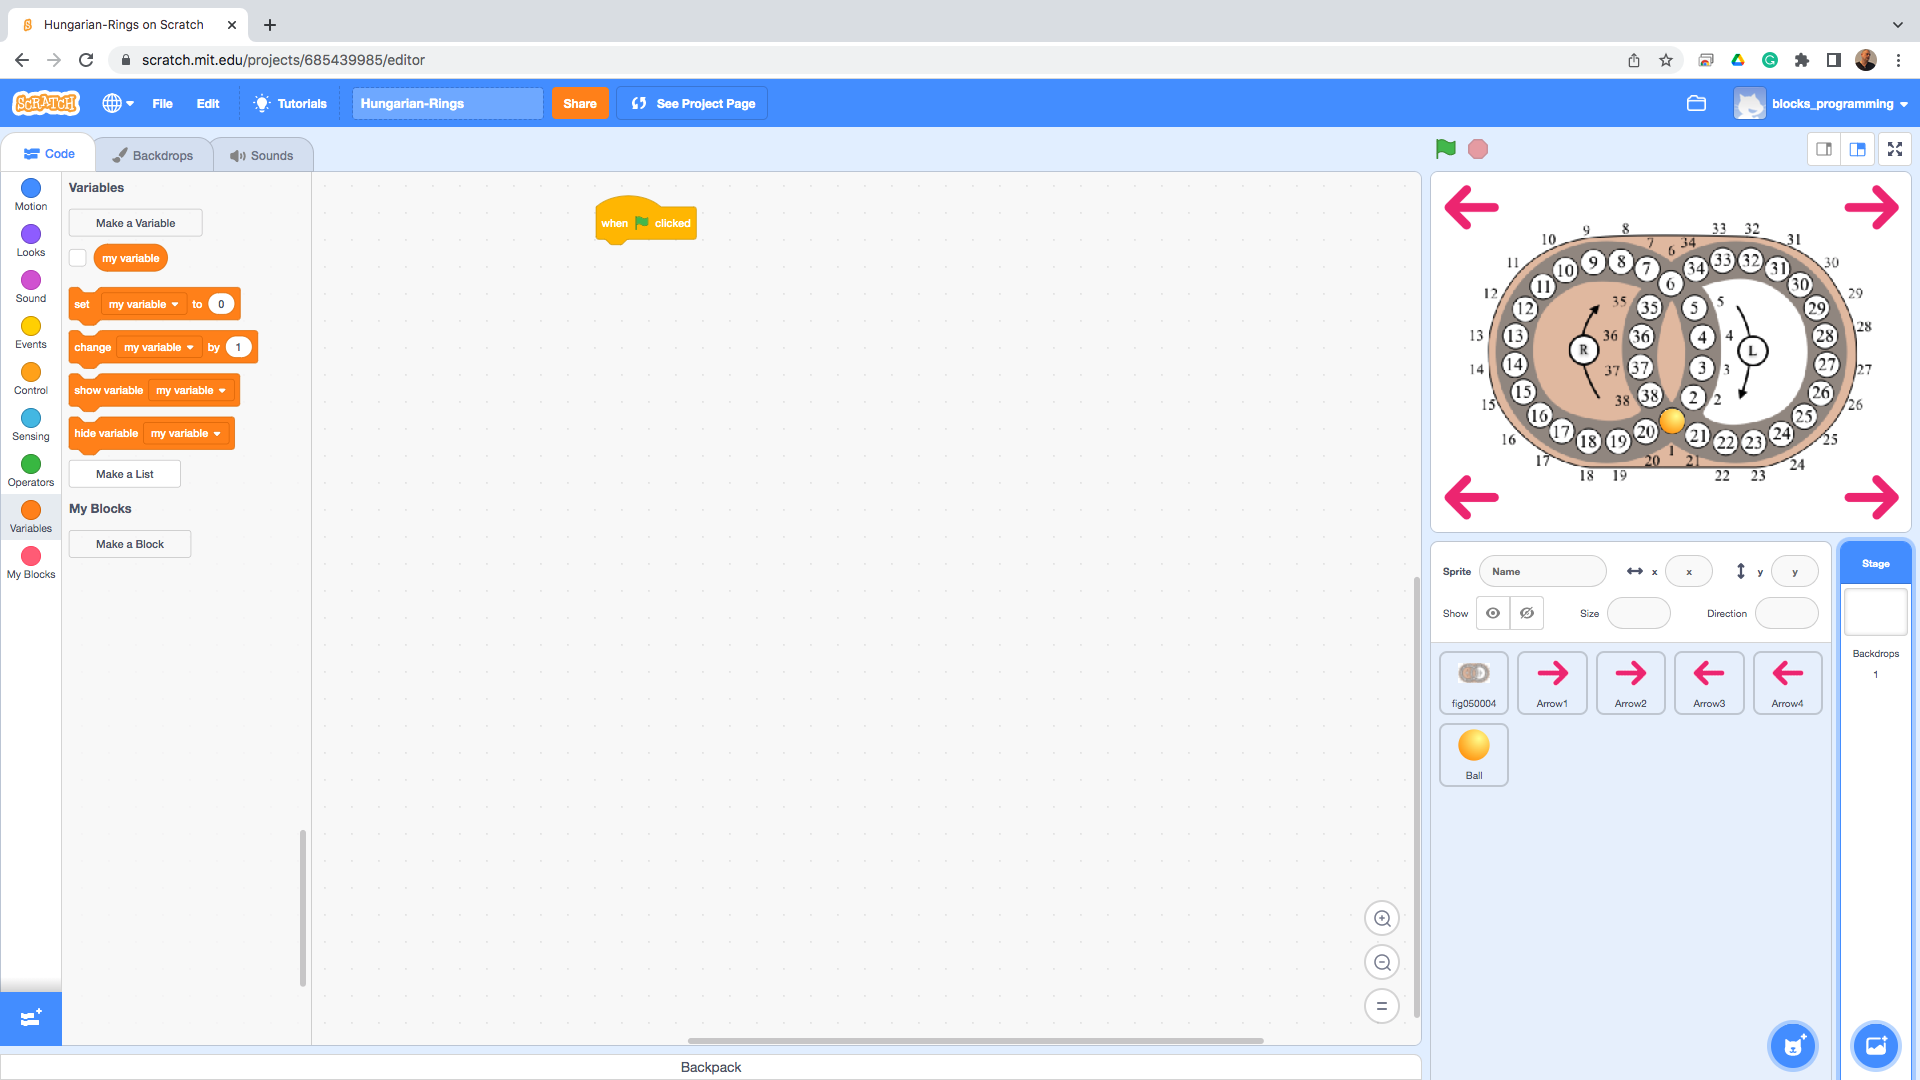
\includegraphics[width=1.0\linewidth,height=0.5\linewidth]{fig050015.png}
   \caption{Start of the game in scene program field}
\label{fig050015}
\end{figure}

For this purpose, a "state" list is created, and the numbers defining the colors of the polka dots will be written into it.

\begin{figure}[H]
   \centering
   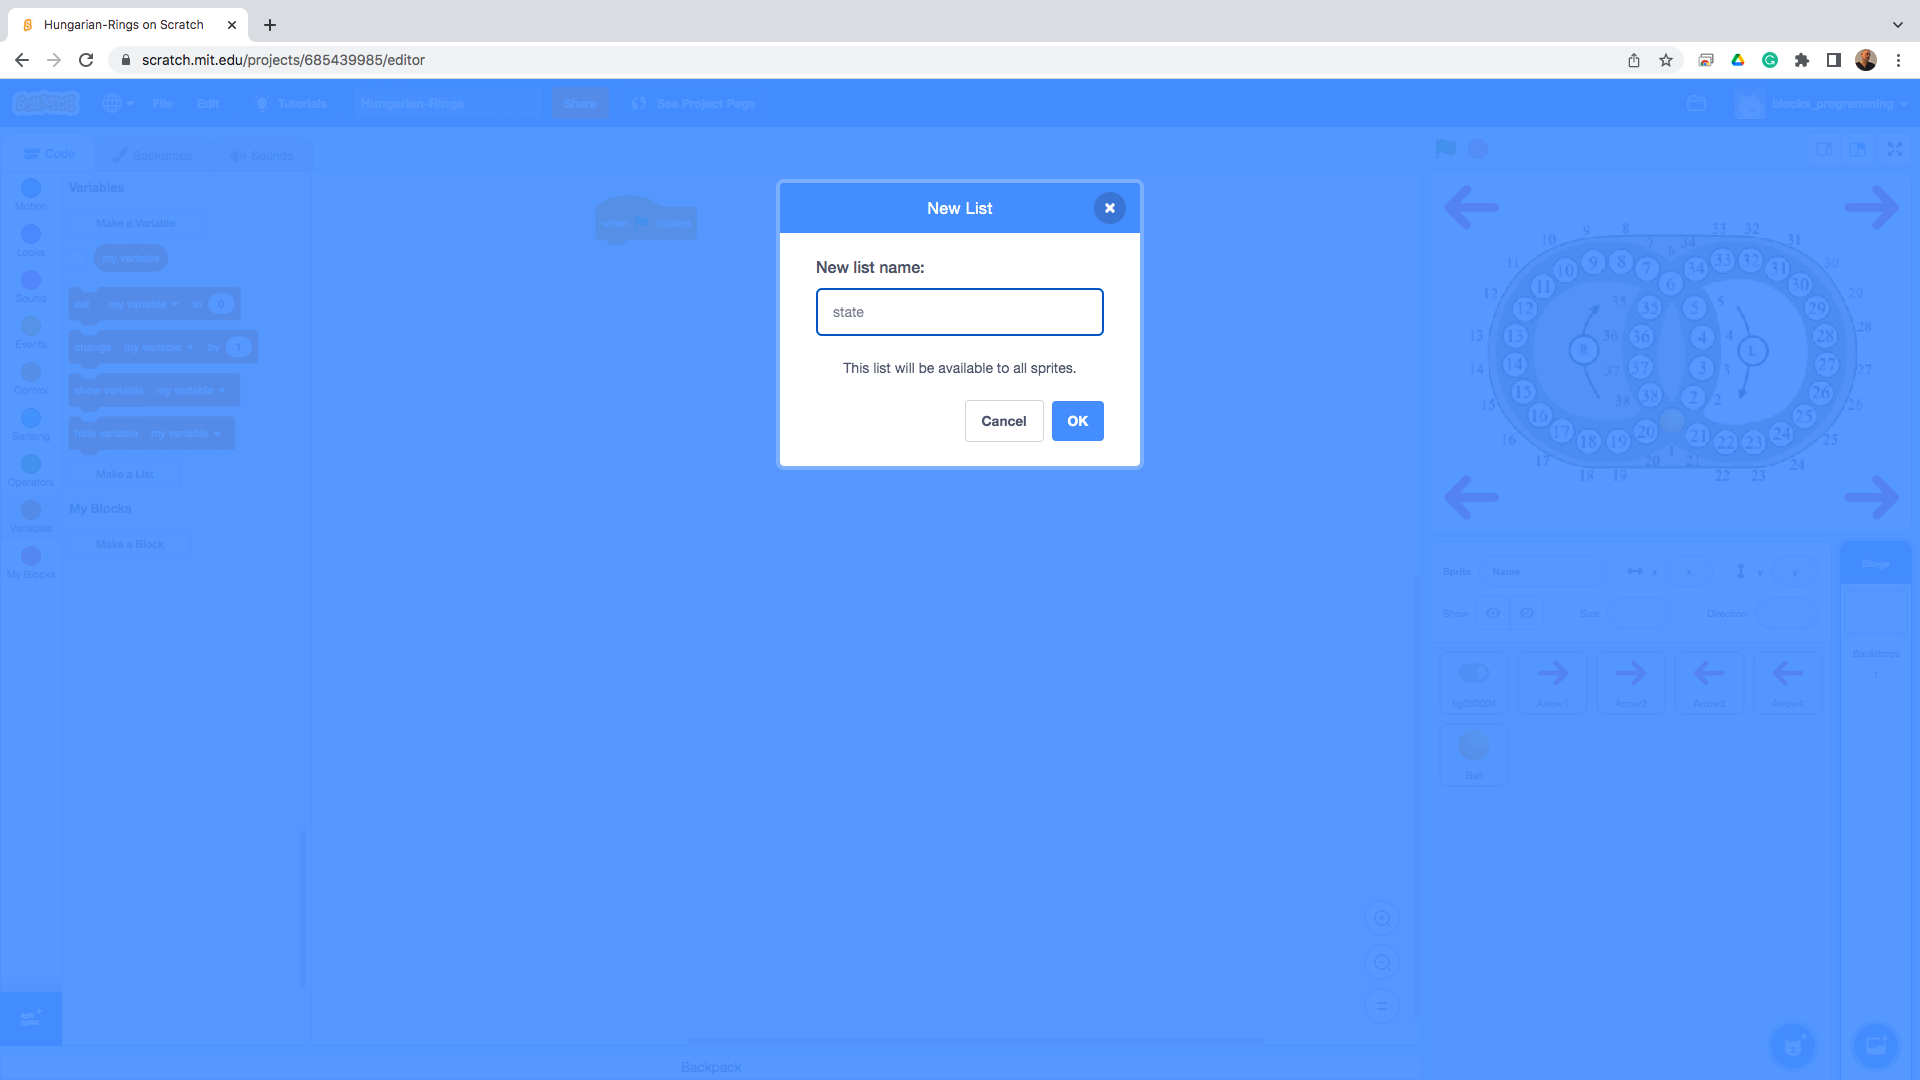
\includegraphics[width=1.0\linewidth,height=0.5\linewidth]{fig050016.png}
   \caption{List of game board status}
\label{fig050016}
\end{figure}

The list's contents are always completely deleted first, so no values from a previous run remain. The first five positions are of the first color (Fig. \ref{fig050017}).

\begin{figure}[H]
   \centering
   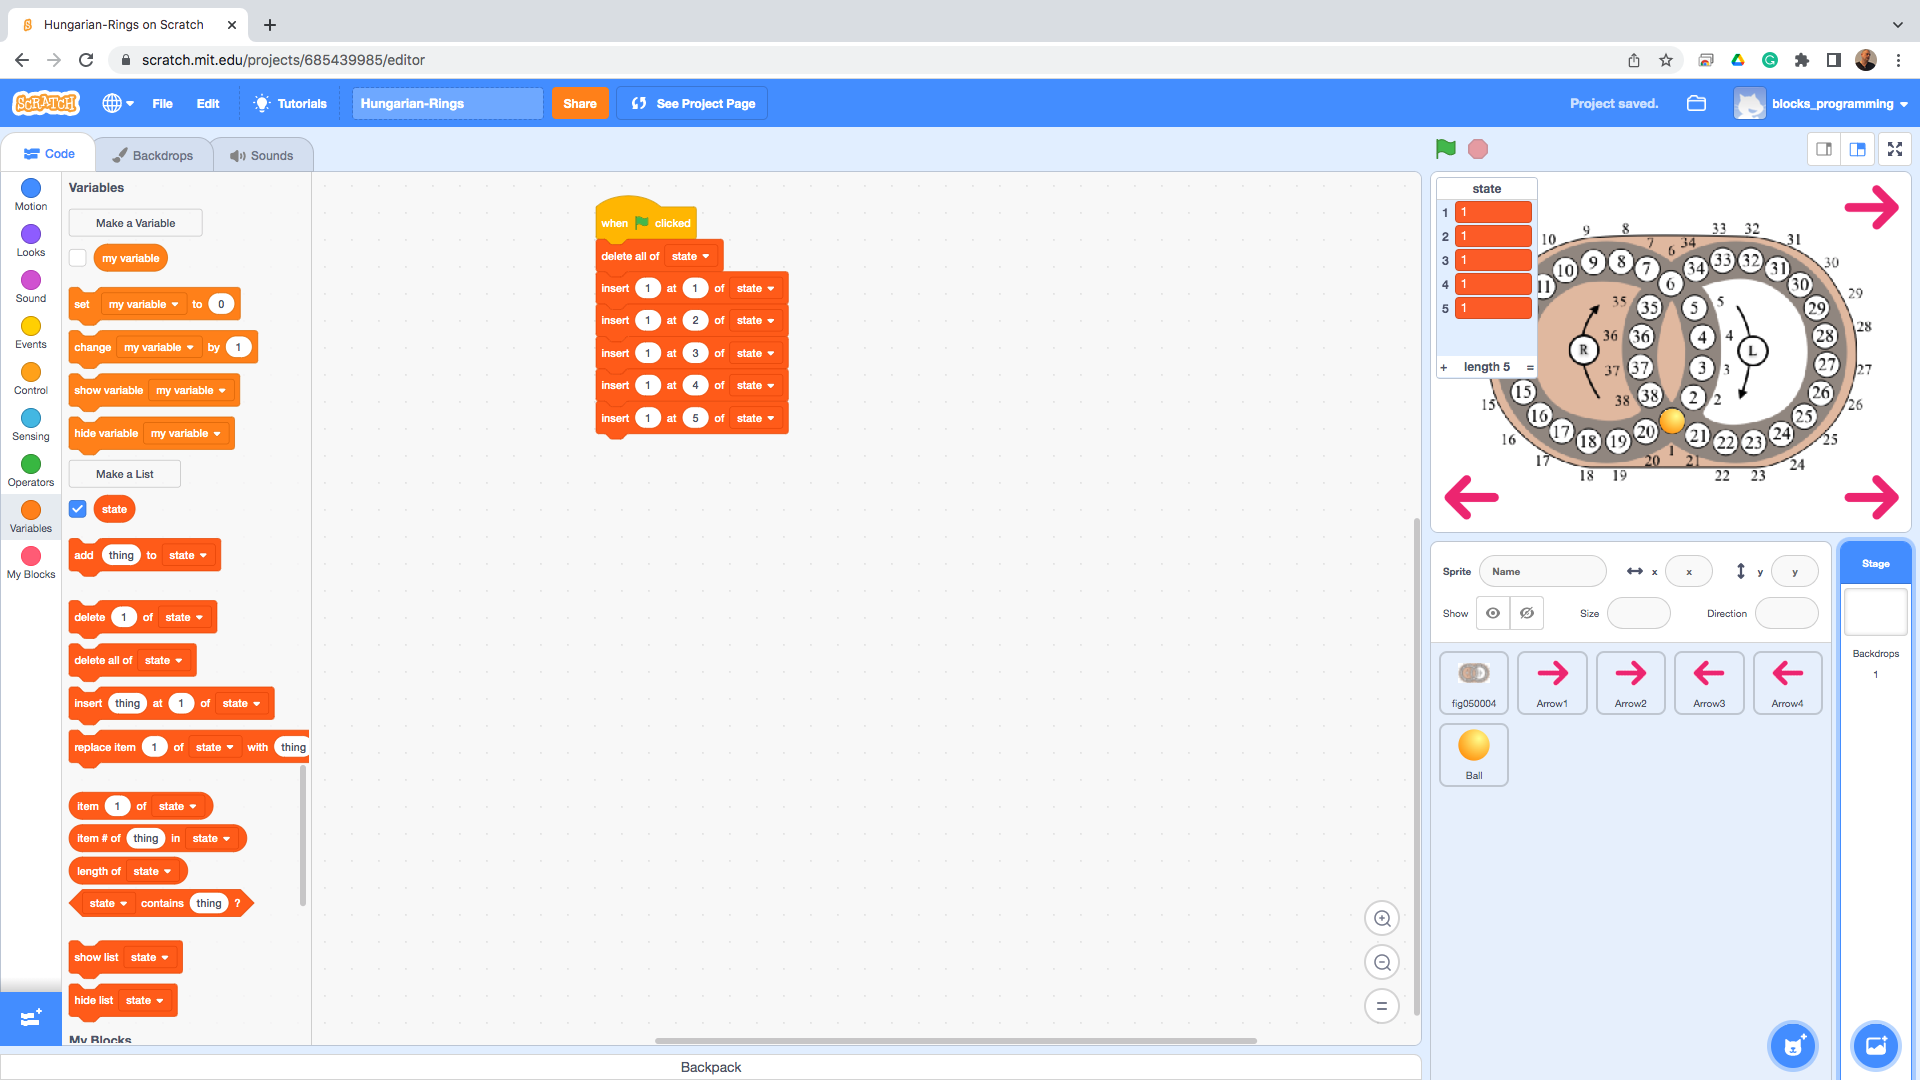
\includegraphics[width=1.0\linewidth,height=0.5\linewidth]{fig050017.png}
   \caption{Color of first five positions}
\label{fig050017}
\end{figure}

The fourth color appears in the sixth position, then from the seventh to the sixteenth position is the second color. Four positions of the first suit follow, and from twenty-one to thirty are positions of the third suit. All other checkers are of the fourth color (Fig. \ref{fig050018}).

\begin{figure}[H]
   \centering
   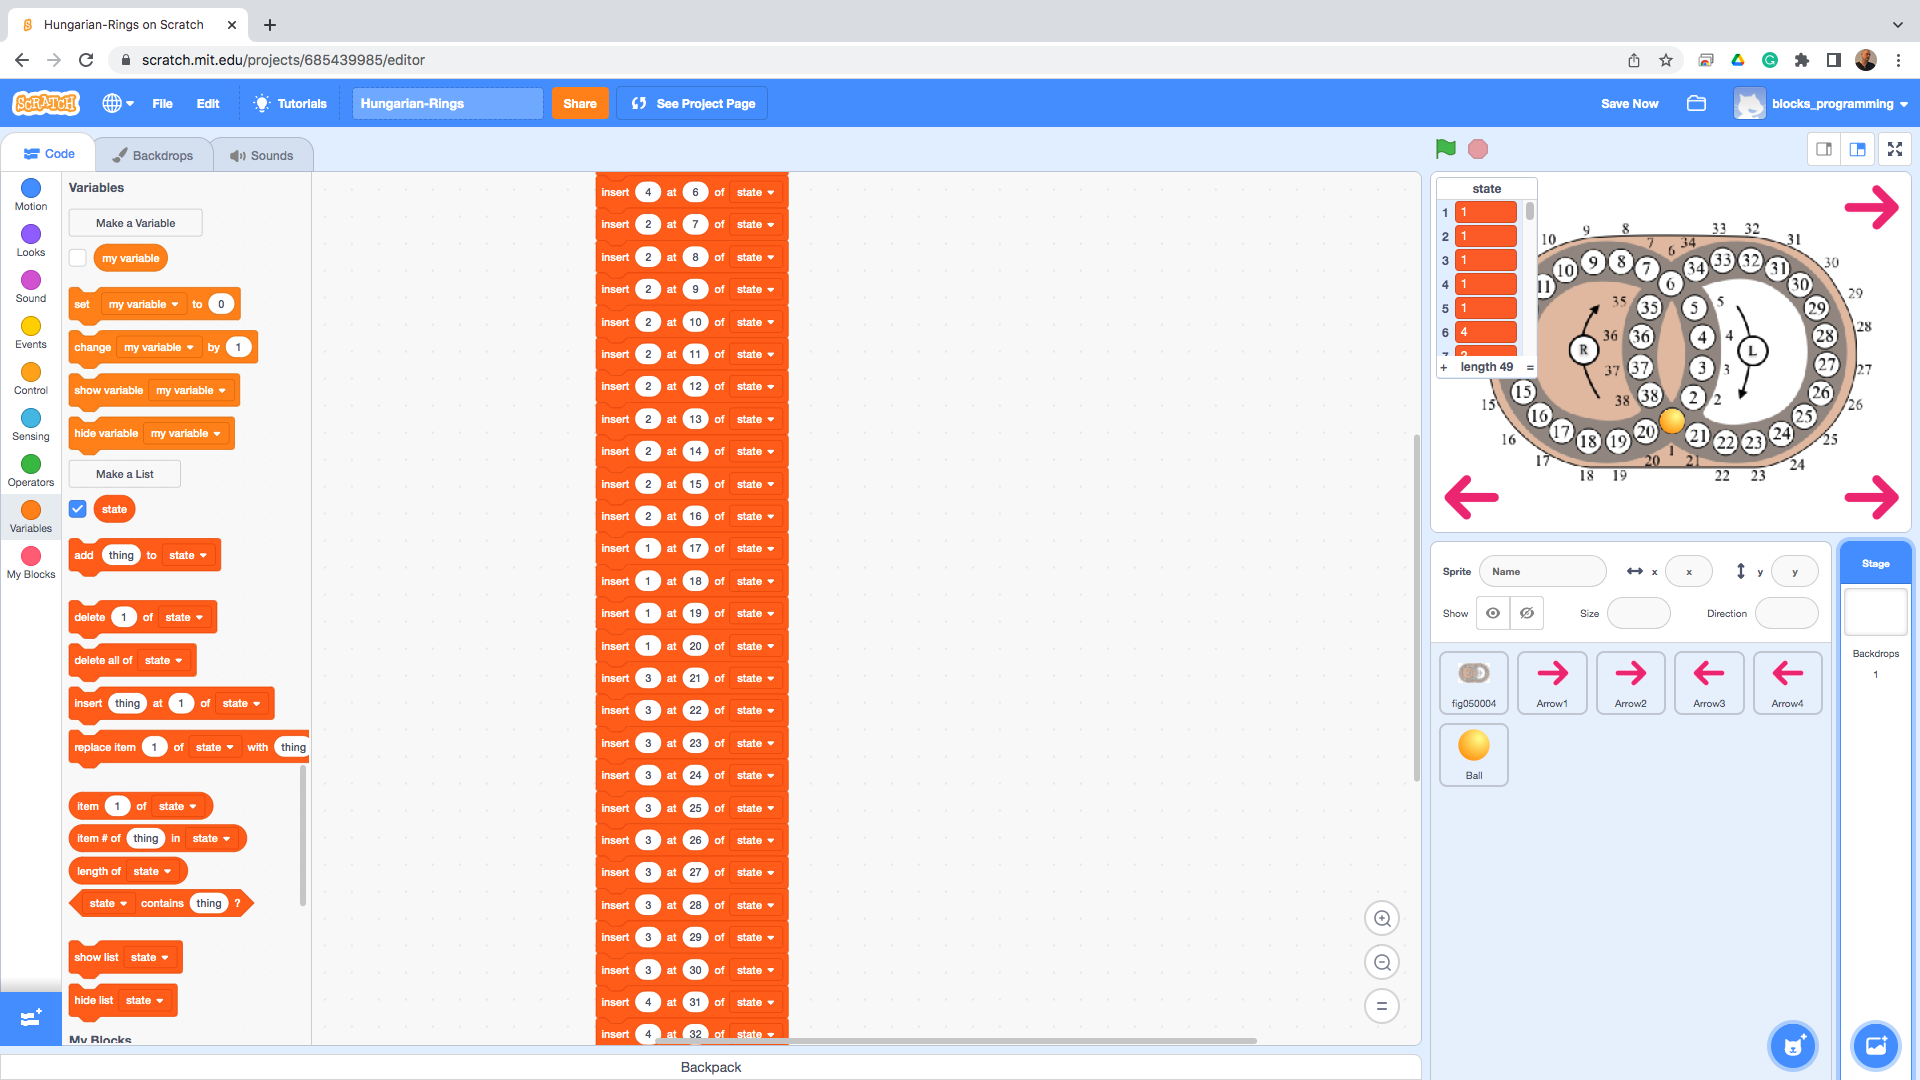
\includegraphics[width=1.0\linewidth,height=0.5\linewidth]{fig050018.png}
   \caption{Overall status by color}
\label{fig050018}
\end{figure}

After a change in the internal state of the list, it is essential to send an update message to all sprites that render the polka dots (Fig. \ref{fig050019}).

\begin{figure}[H]
   \centering
   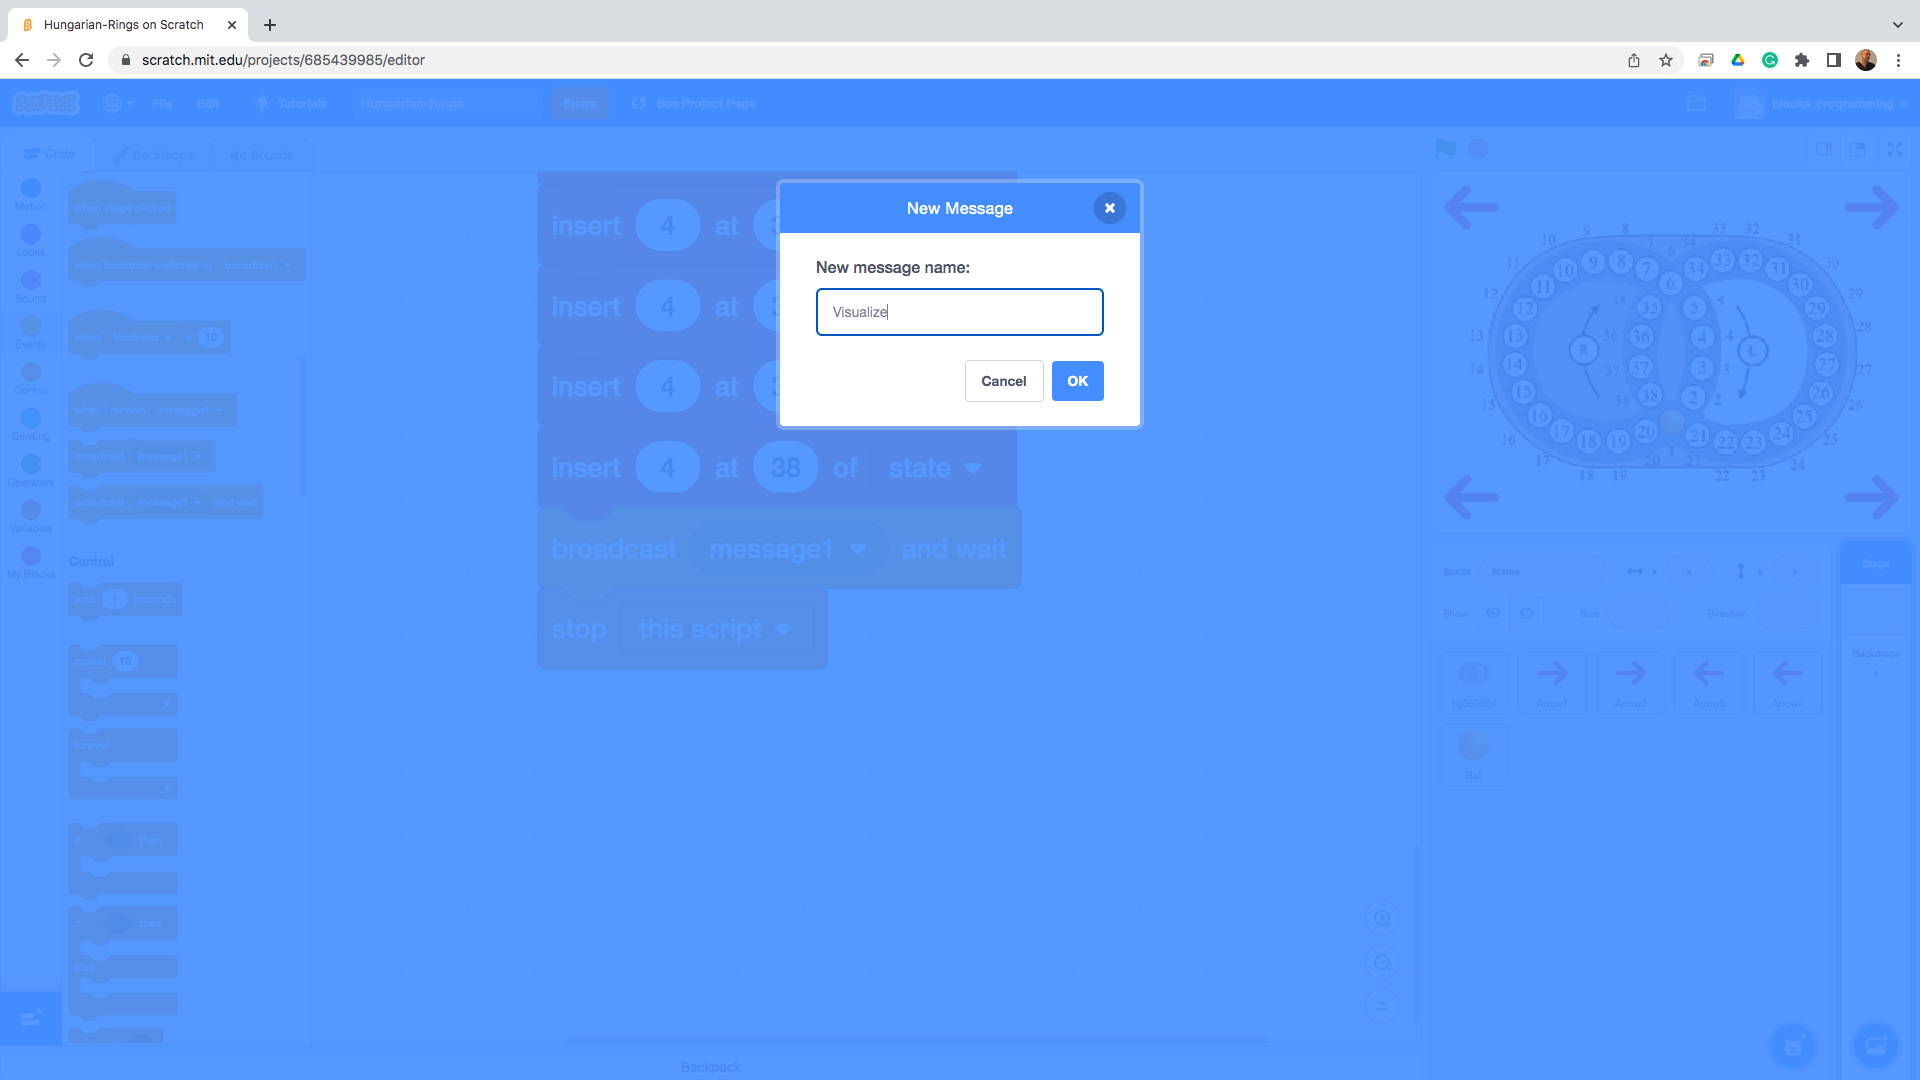
\includegraphics[width=1.0\linewidth,height=0.5\linewidth]{fig050019.png}
   \caption{Preview message}
\label{fig050019}
\end{figure}

The message is sent with a command that waits for its execution (Fig. \ref{fig050020}). Each of the 38 beads will subscribe to receive this message.

\begin{figure}[H]
   \centering
   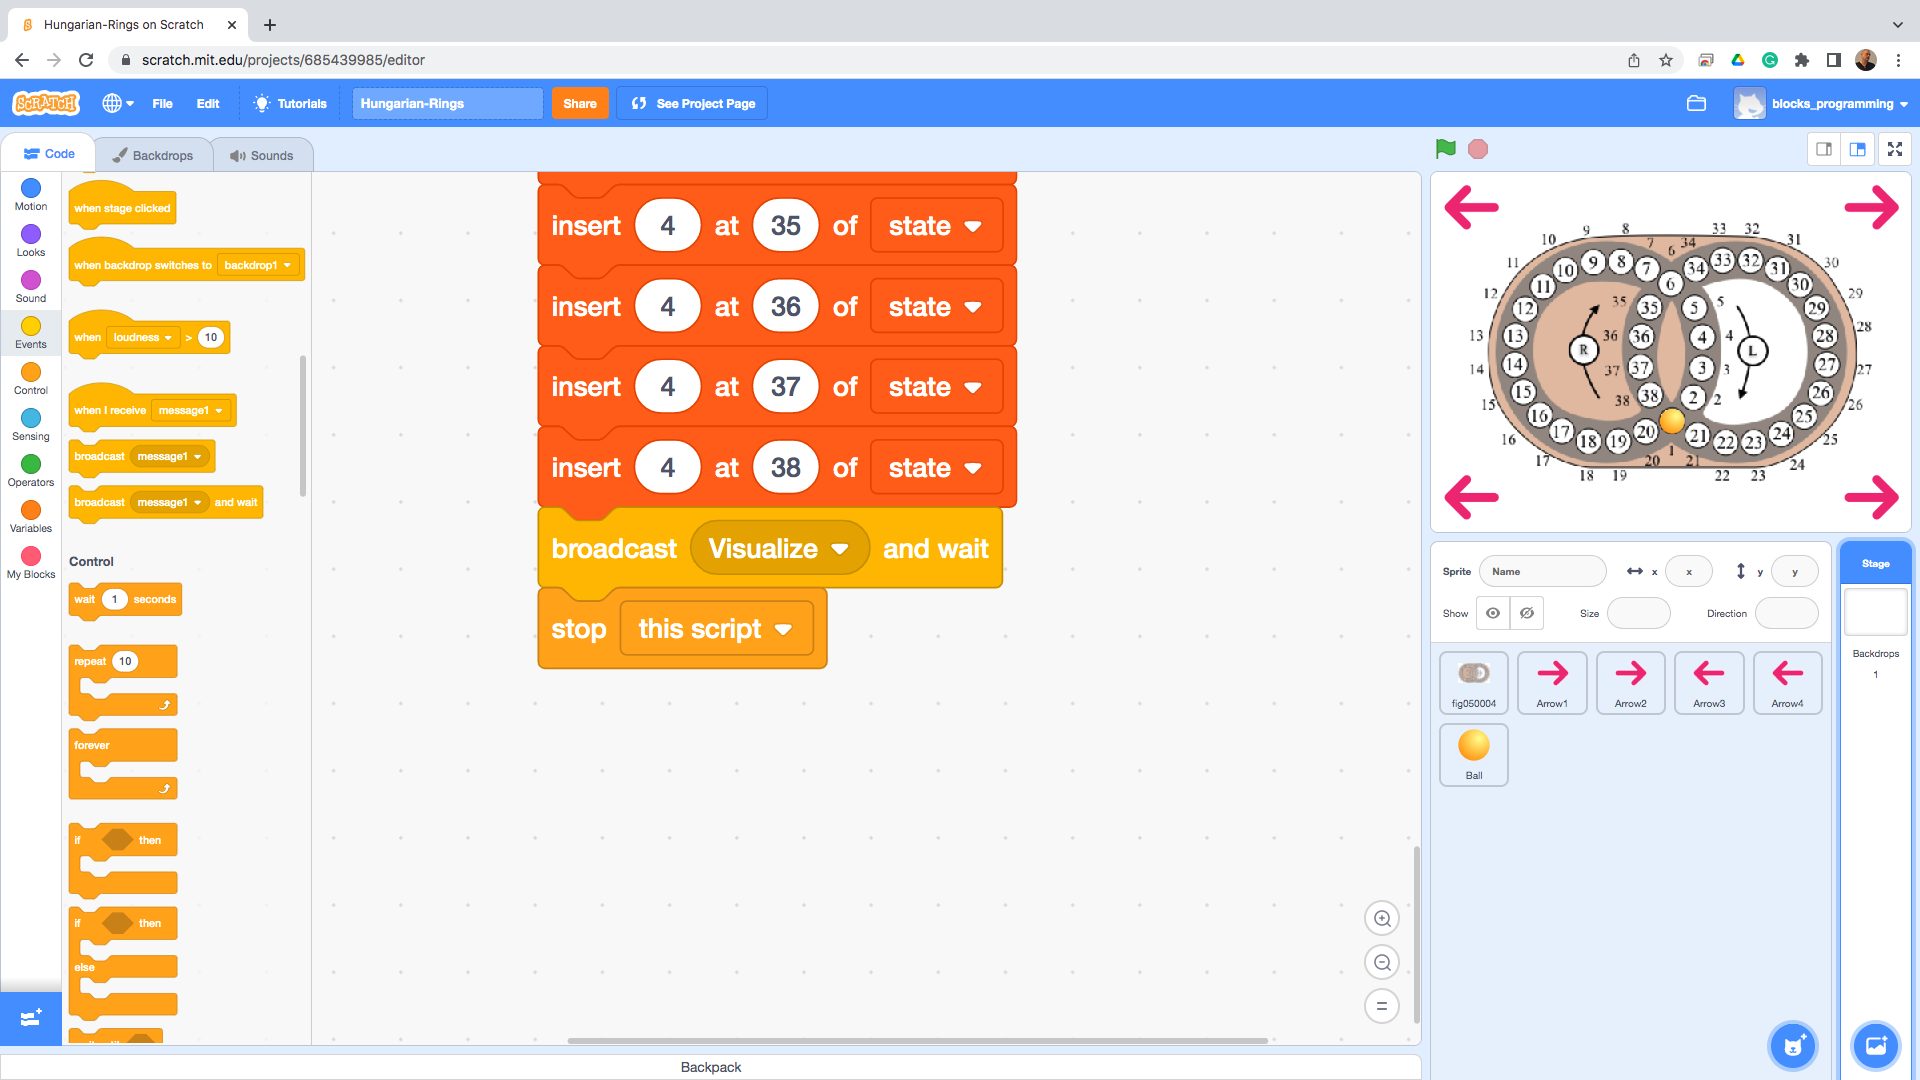
\includegraphics[width=1.0\linewidth,height=0.5\linewidth]{fig050020.png}
   \caption{Sending on hold}
\label{fig050020}
\end{figure}

The code that will listen for a draw message should be compiled before copying the first pool so that it is multiplied another 37 times. First, this code is written so that it is multiplied 37 times when duplicating the sprite. A pool with number one makes four checks on list item number one. According to the number in the list, one of the four possible colors is selected (Fig. \ref{fig050021}).

\begin{figure}[H]
   \centering
   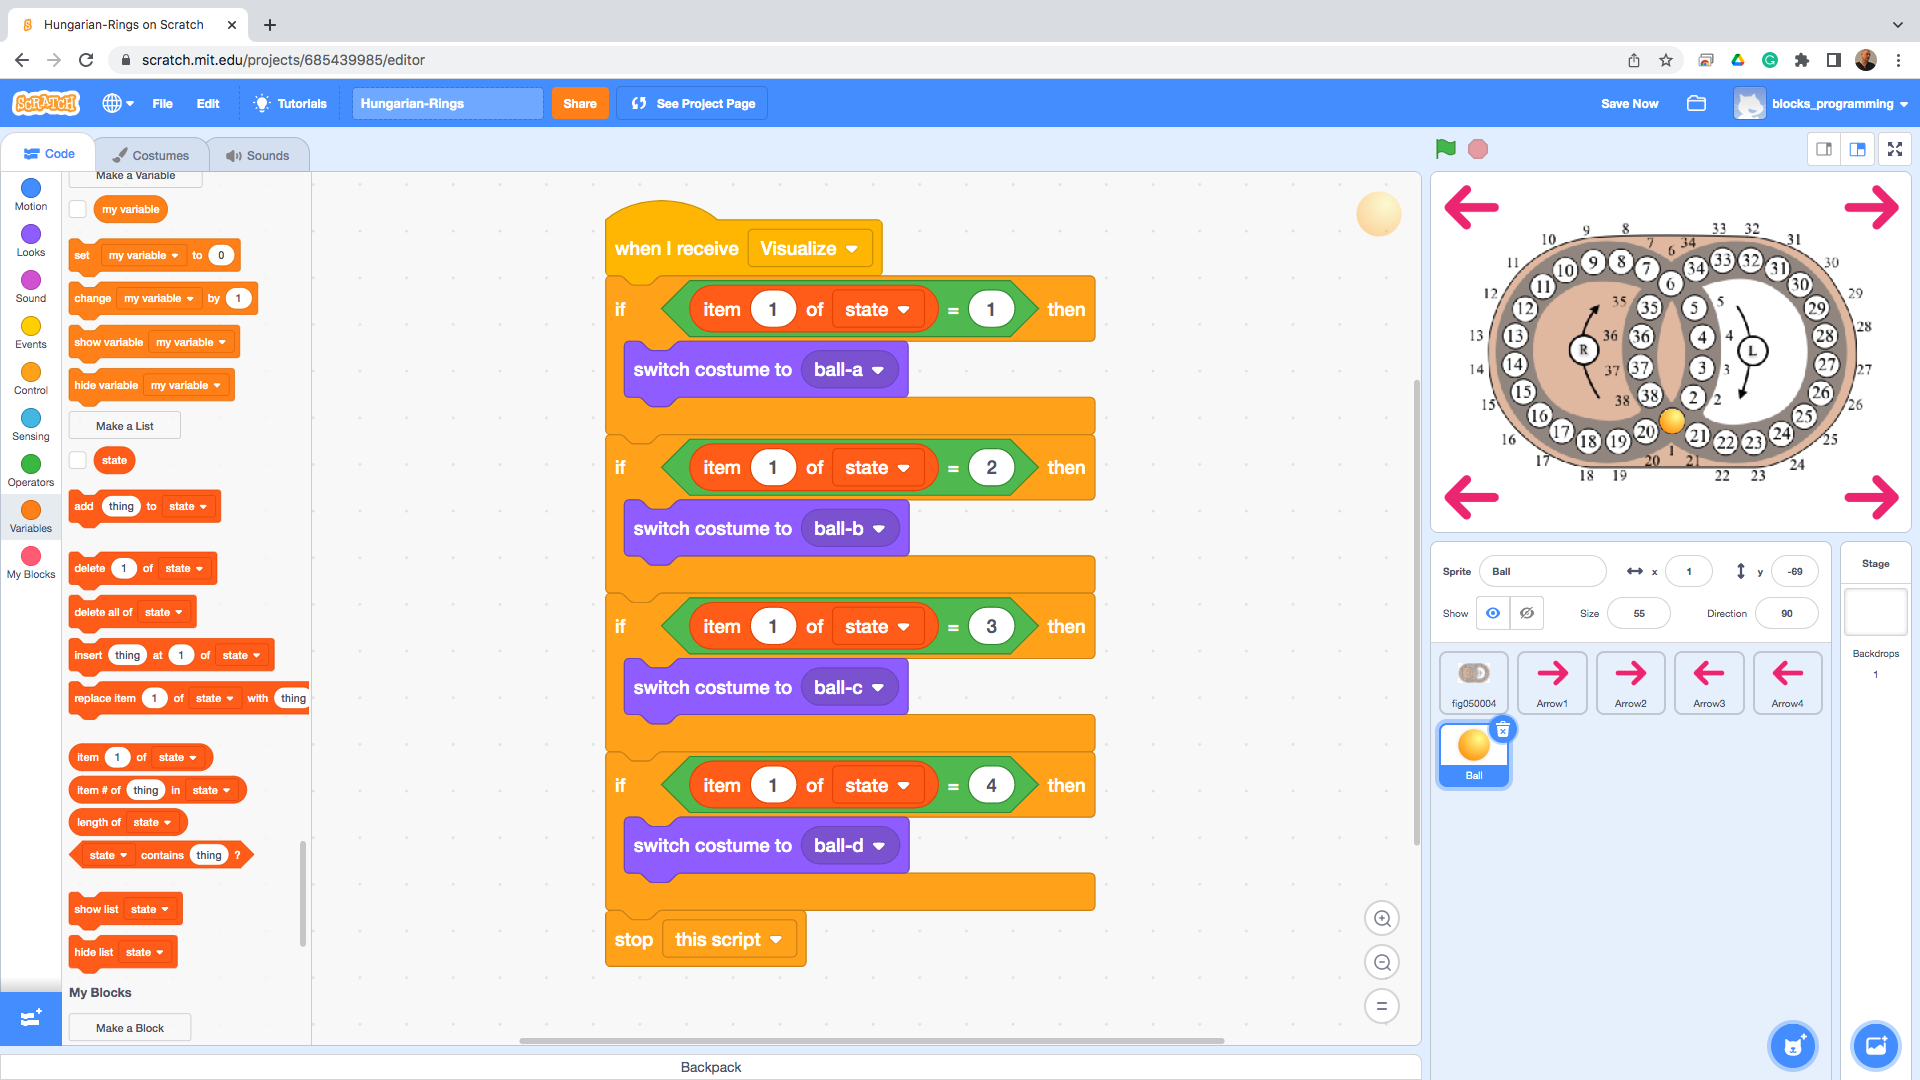
\includegraphics[width=1.0\linewidth,height=0.5\linewidth]{fig050021.png}
   \caption{Instructions for redrawing the pool}
\label{fig050021}
\end{figure}

The first pool thus prepared can be duplicated and spread over the entire scheme, taking into account the colors of the individual positions (Fig. \ref{fig050022}).

\begin{figure}[H]
   \centering
   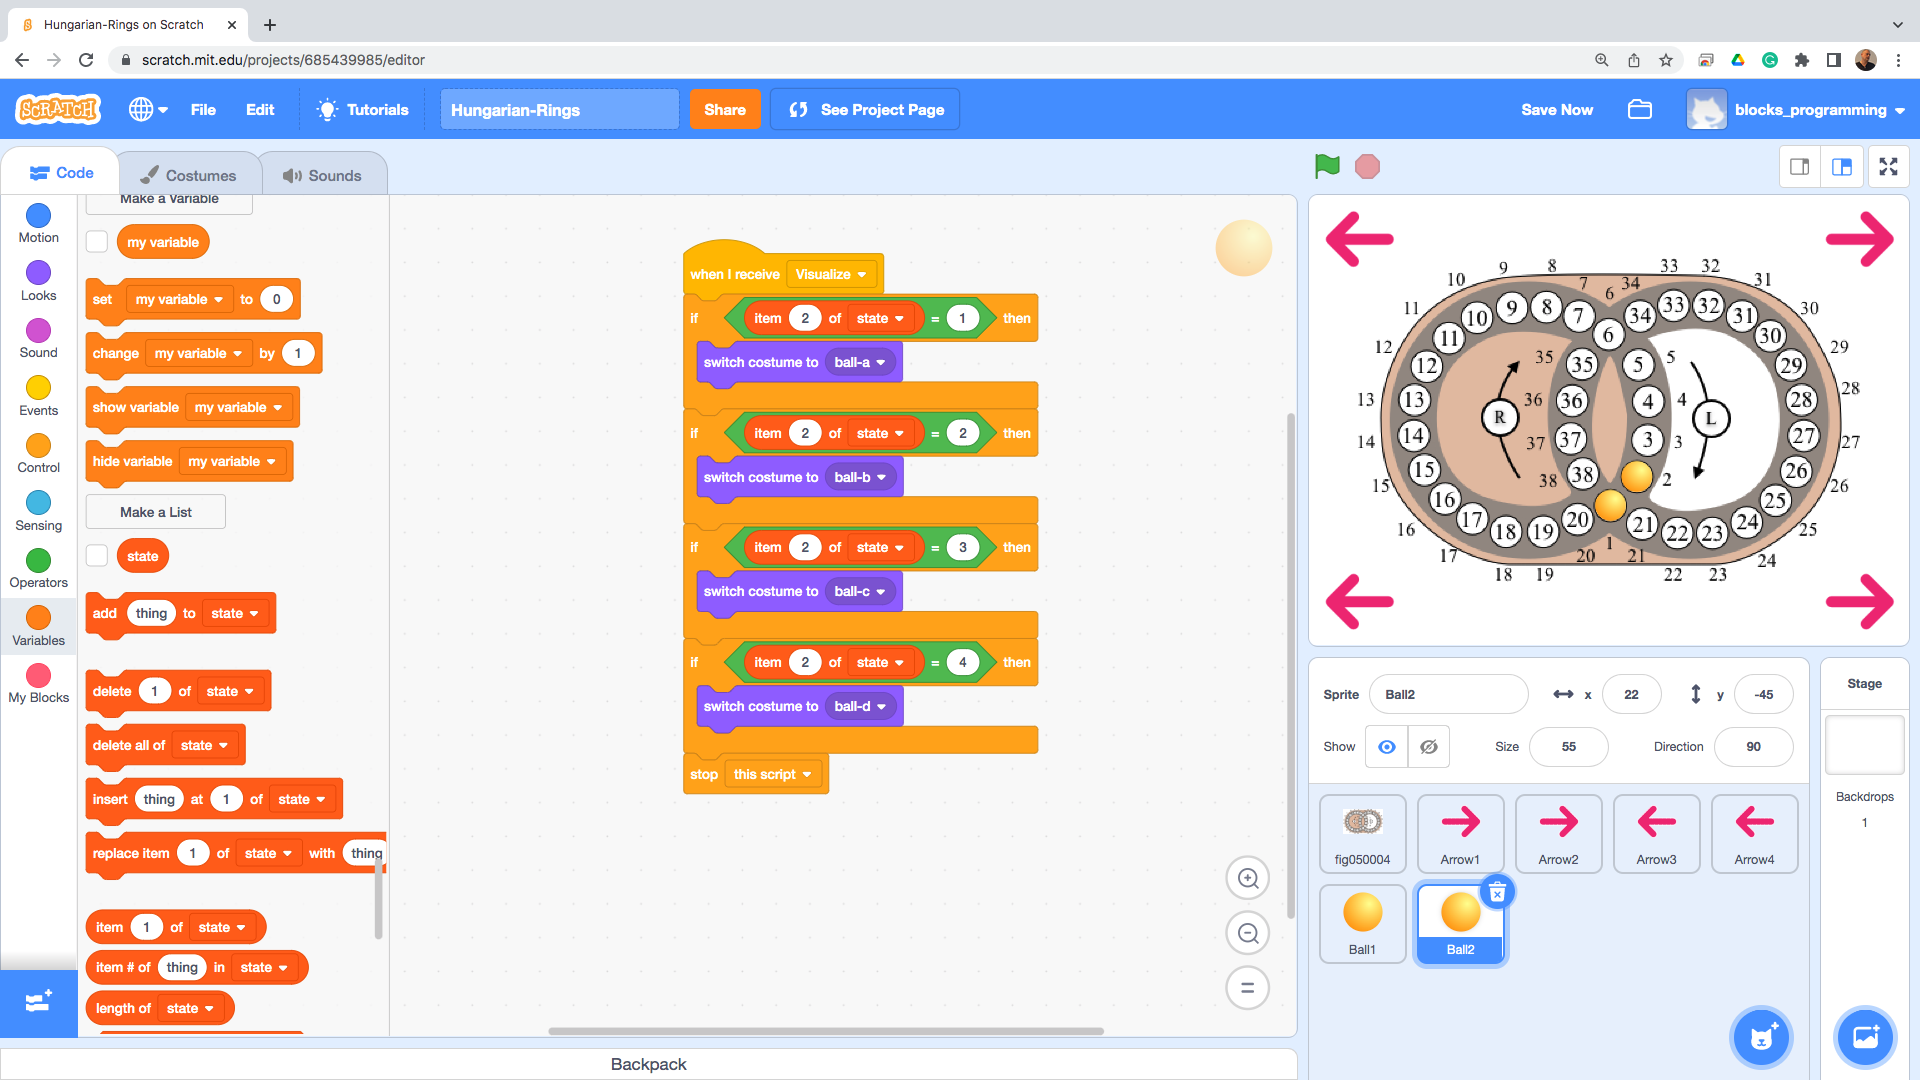
\includegraphics[width=1.0\linewidth,height=0.5\linewidth]{fig050022.png}
   \caption{Duplicate pool}
\label{fig050022}
\end{figure}

The two rings are clearly formed when arranging all 38 checkers on the game diagram (Fig. \ref{fig050023}).

\begin{figure}[H]
   \centering
   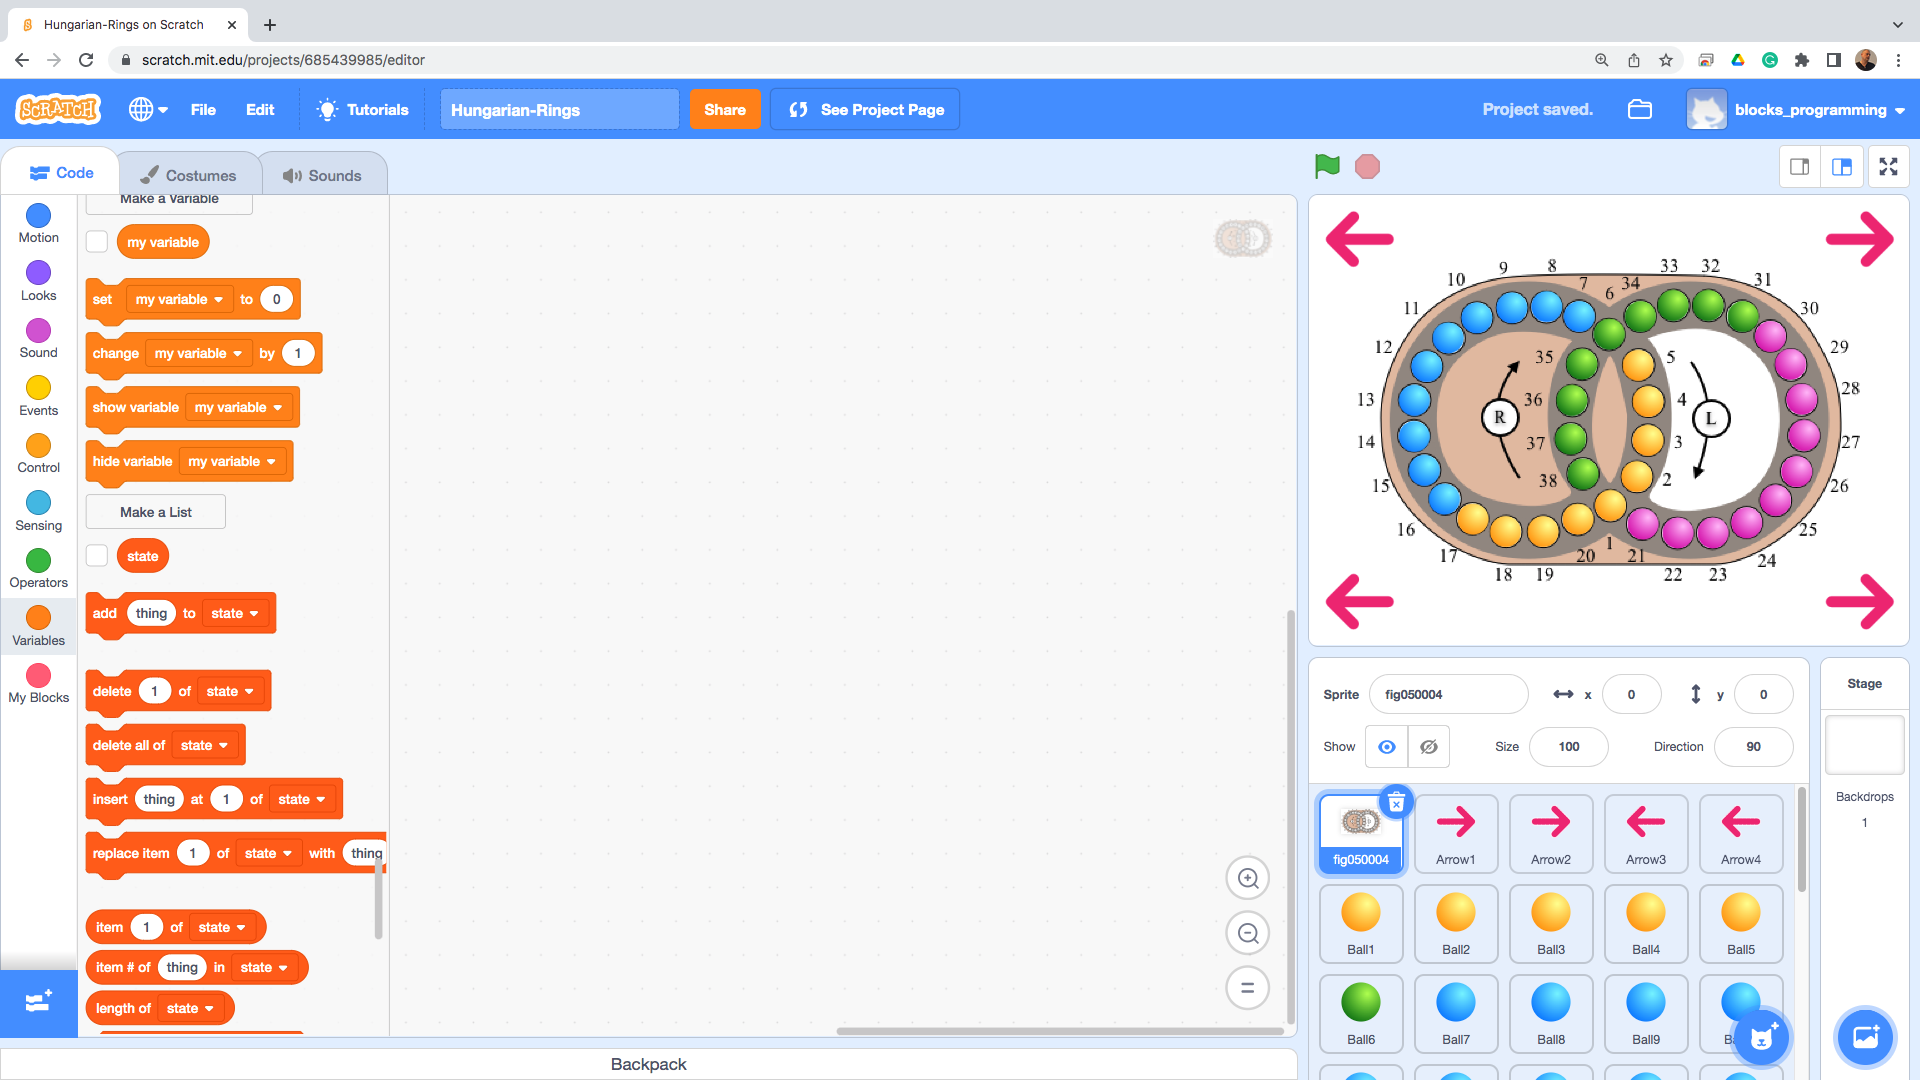
\includegraphics[width=1.0\linewidth,height=0.5\linewidth]{fig050023.png}
   \caption{Duplicate pool}
\label{fig050023}
\end{figure}

At this stage, the game plan is only an aid (Fig. \ref{fig050024}). When the numbering is removed, the same image can be used for the background of the two checker rings.

\begin{figure}[H]
   \centering
   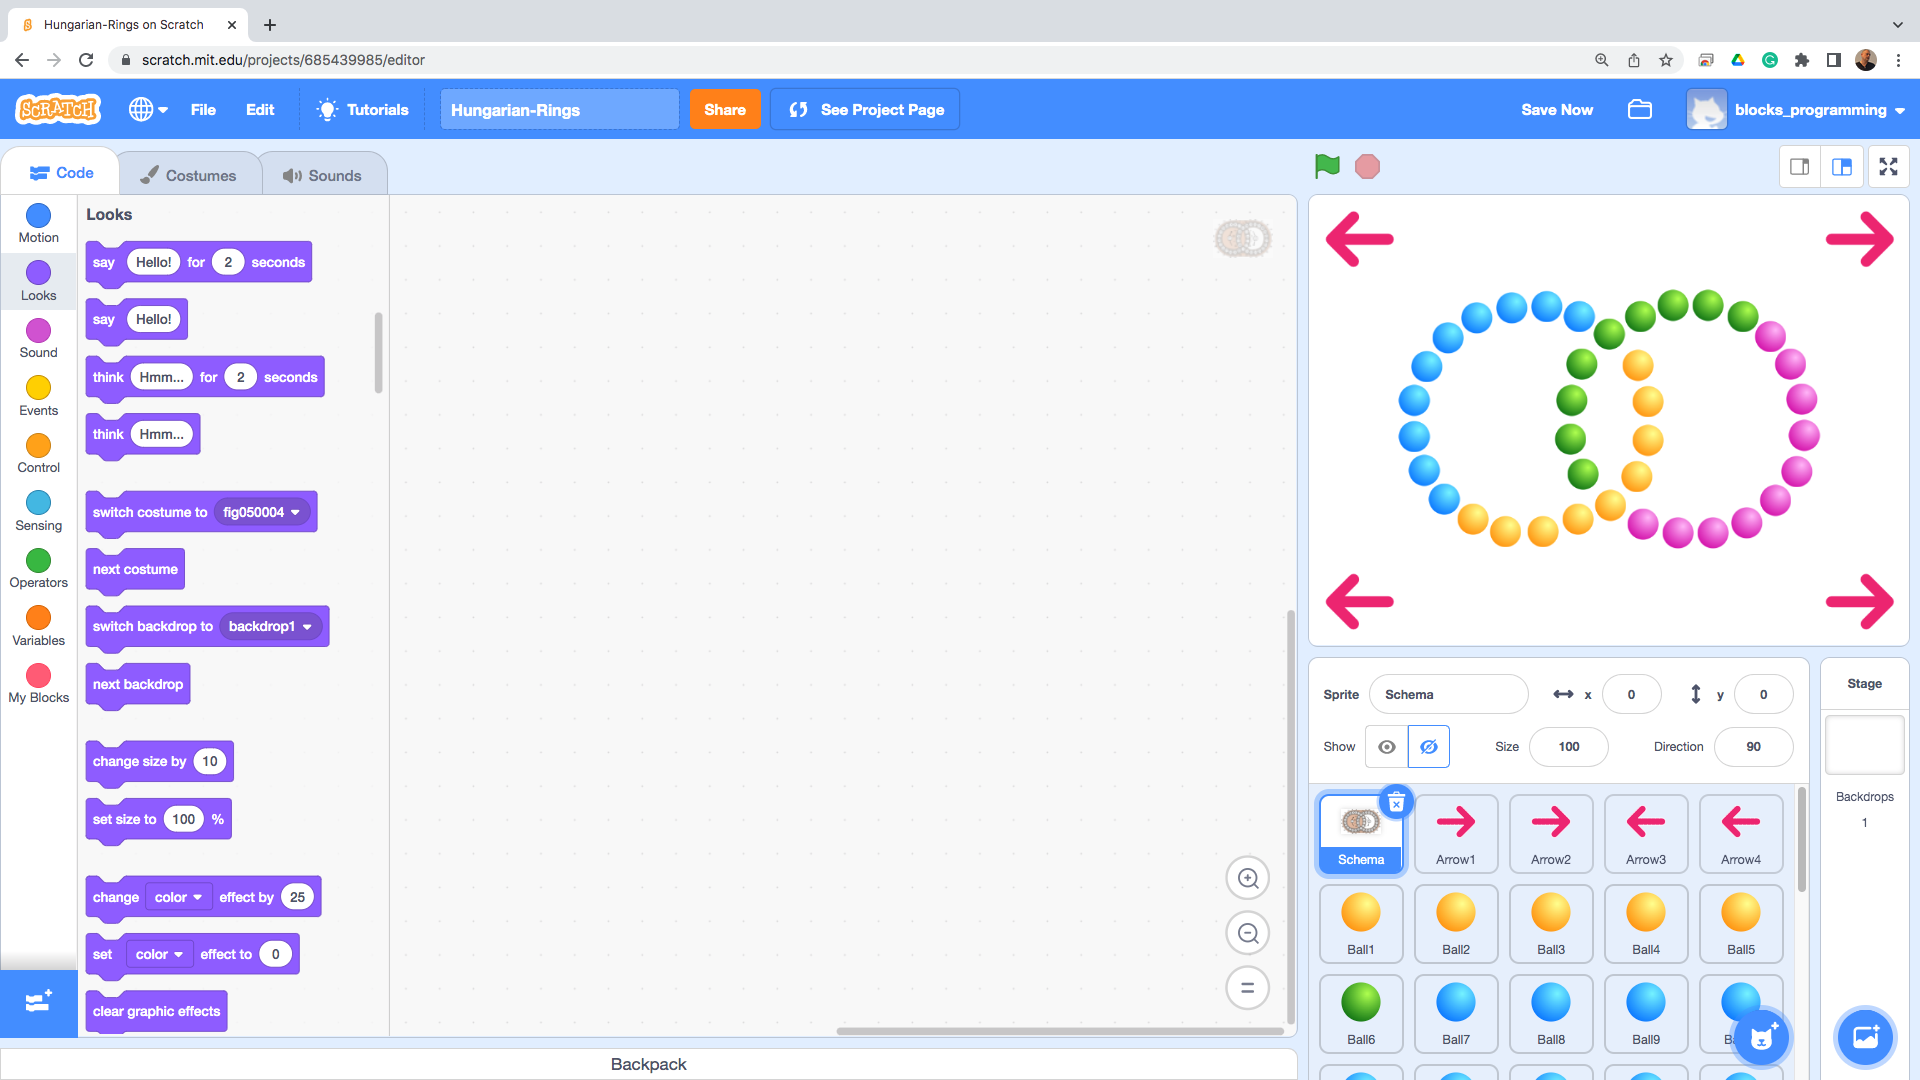
\includegraphics[width=1.0\linewidth,height=0.5\linewidth]{fig050024.png}
   \caption{Remove Scheme}
\label{fig050024}
\end{figure}

\section{Algorithms for Manipulation of the Playing Field}

Pressing the first arrow (upper-right) first propagates a message to perform a rotation in the right ring, clockwise (Fig. \ref{fig050025}). A message is then propagated to refresh the entire visual space.

\begin{figure}[H]
   \centering
   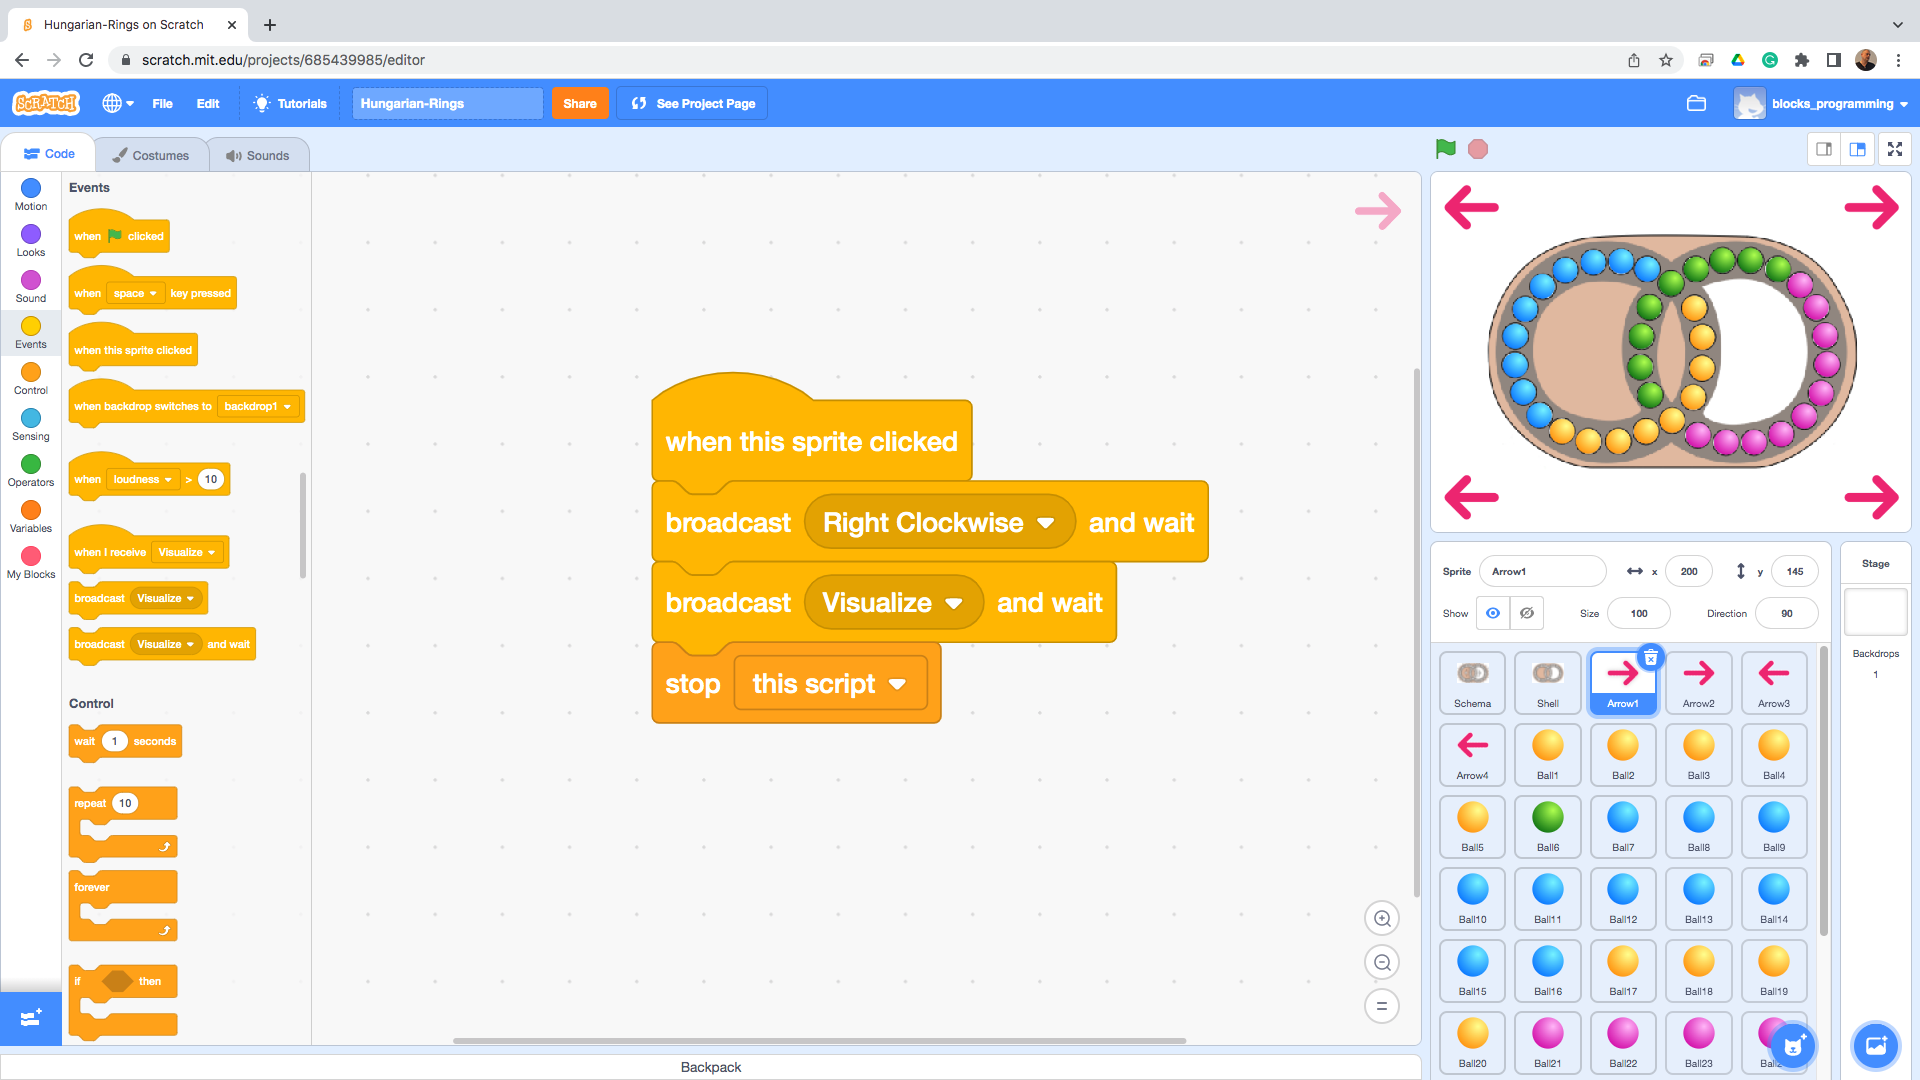
\includegraphics[width=1.0\linewidth,height=0.5\linewidth]{fig050025.png}
   \caption{Rotation and drawing message}
\label{fig050025}
\end{figure}

In an absolutely analogous way, messages are sent from the other three hands, with the messages indicating the ring and the direction of rotation. After the initialization of the color list, a preview follows, then a small interval is given so that the user can see the initial state and a message is sent to shuffle the puzzle (Fig. \ref{fig050026}).

\begin{figure}[H]
   \centering
   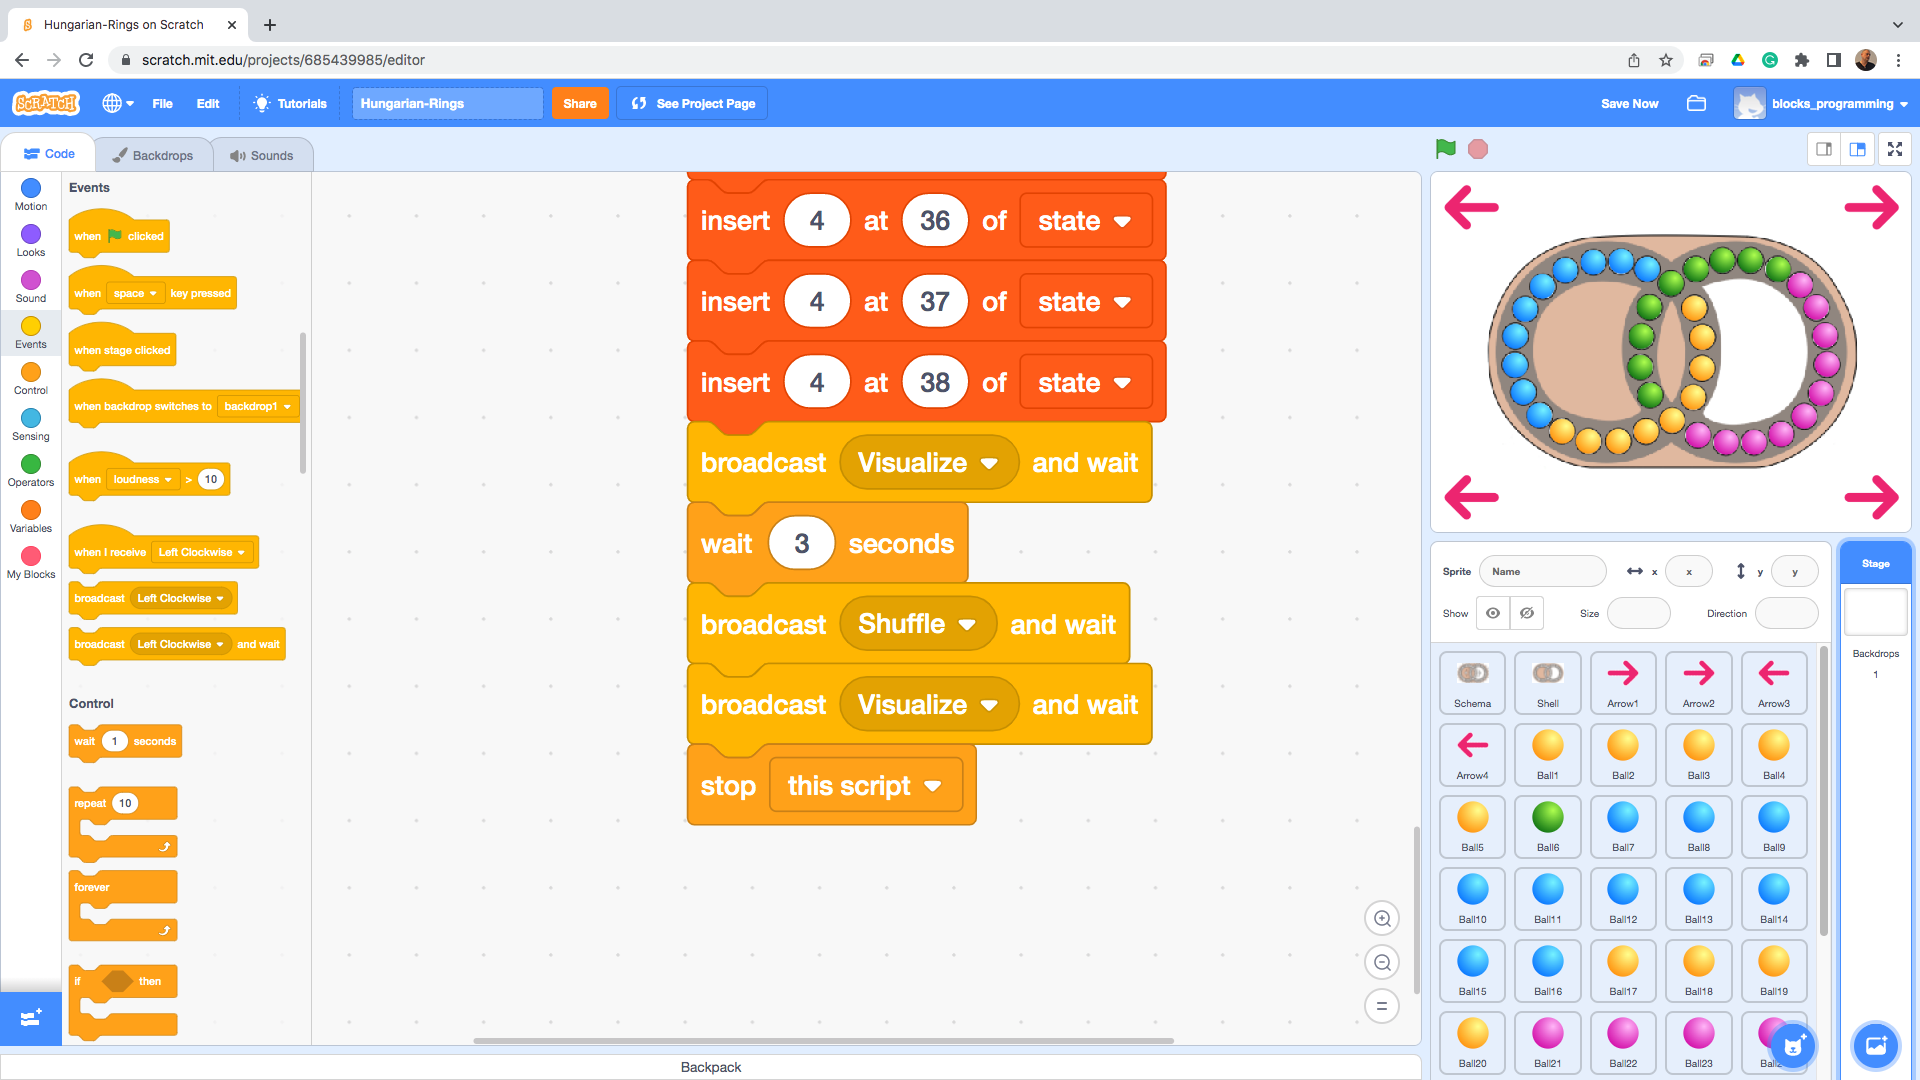
\includegraphics[width=1.0\linewidth,height=0.5\linewidth]{fig050026.png}
   \caption{Send shuffle message}
\label{fig050026}
\end{figure}

Shuffling the puzzle can happen in many ways, but randomly calling the four rotation possibilities is the most successful. This algorithm will also be assembled in the main scene space, not as code for some of the sprites. The algorithm starts upon receiving the shuffle message. Since the checkers are 38 in number, statistically, each one can be given a chance to move 10 times on average. This suggests that the total number of random moves can be determined to be 380, which is 38 times 10 (Fig. \ref{fig050027}).

\begin{figure}[H]
   \centering
   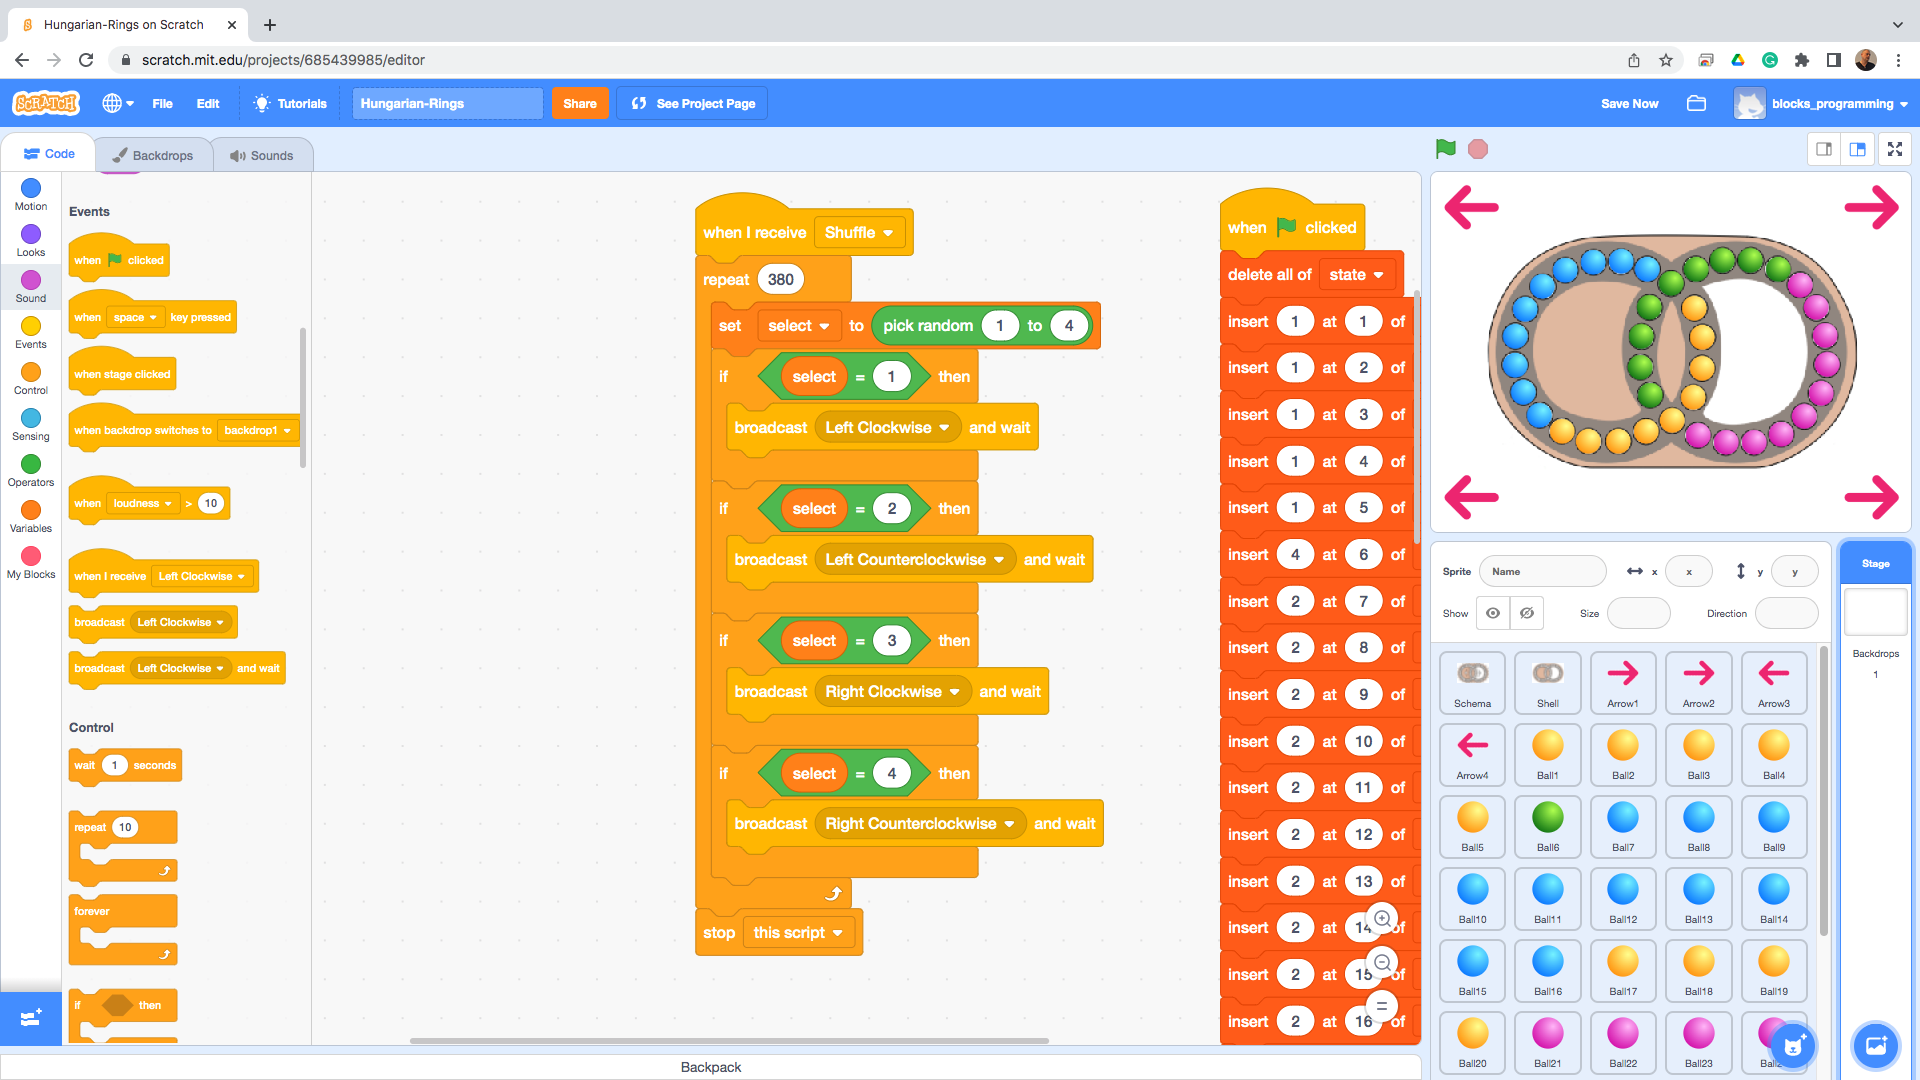
\includegraphics[width=1.0\linewidth,height=0.5\linewidth]{fig050027.png}
   \caption{Shuffling Algorithm}
\label{fig050027}
\end{figure}

The ring rotation instructions will also be placed in the stage space. Each of the four arrows sends an appropriate message. The intercepted rotation message should change the list's contents to reflect the desired rotation. The game board is beneficial for getting the permutations right because it tells you which number should go where.

The rotation of the left ring clockwise is performed with the following sequence of actions (Fig. \ref{fig050028}).

\begin{figure}[H]
   \centering
   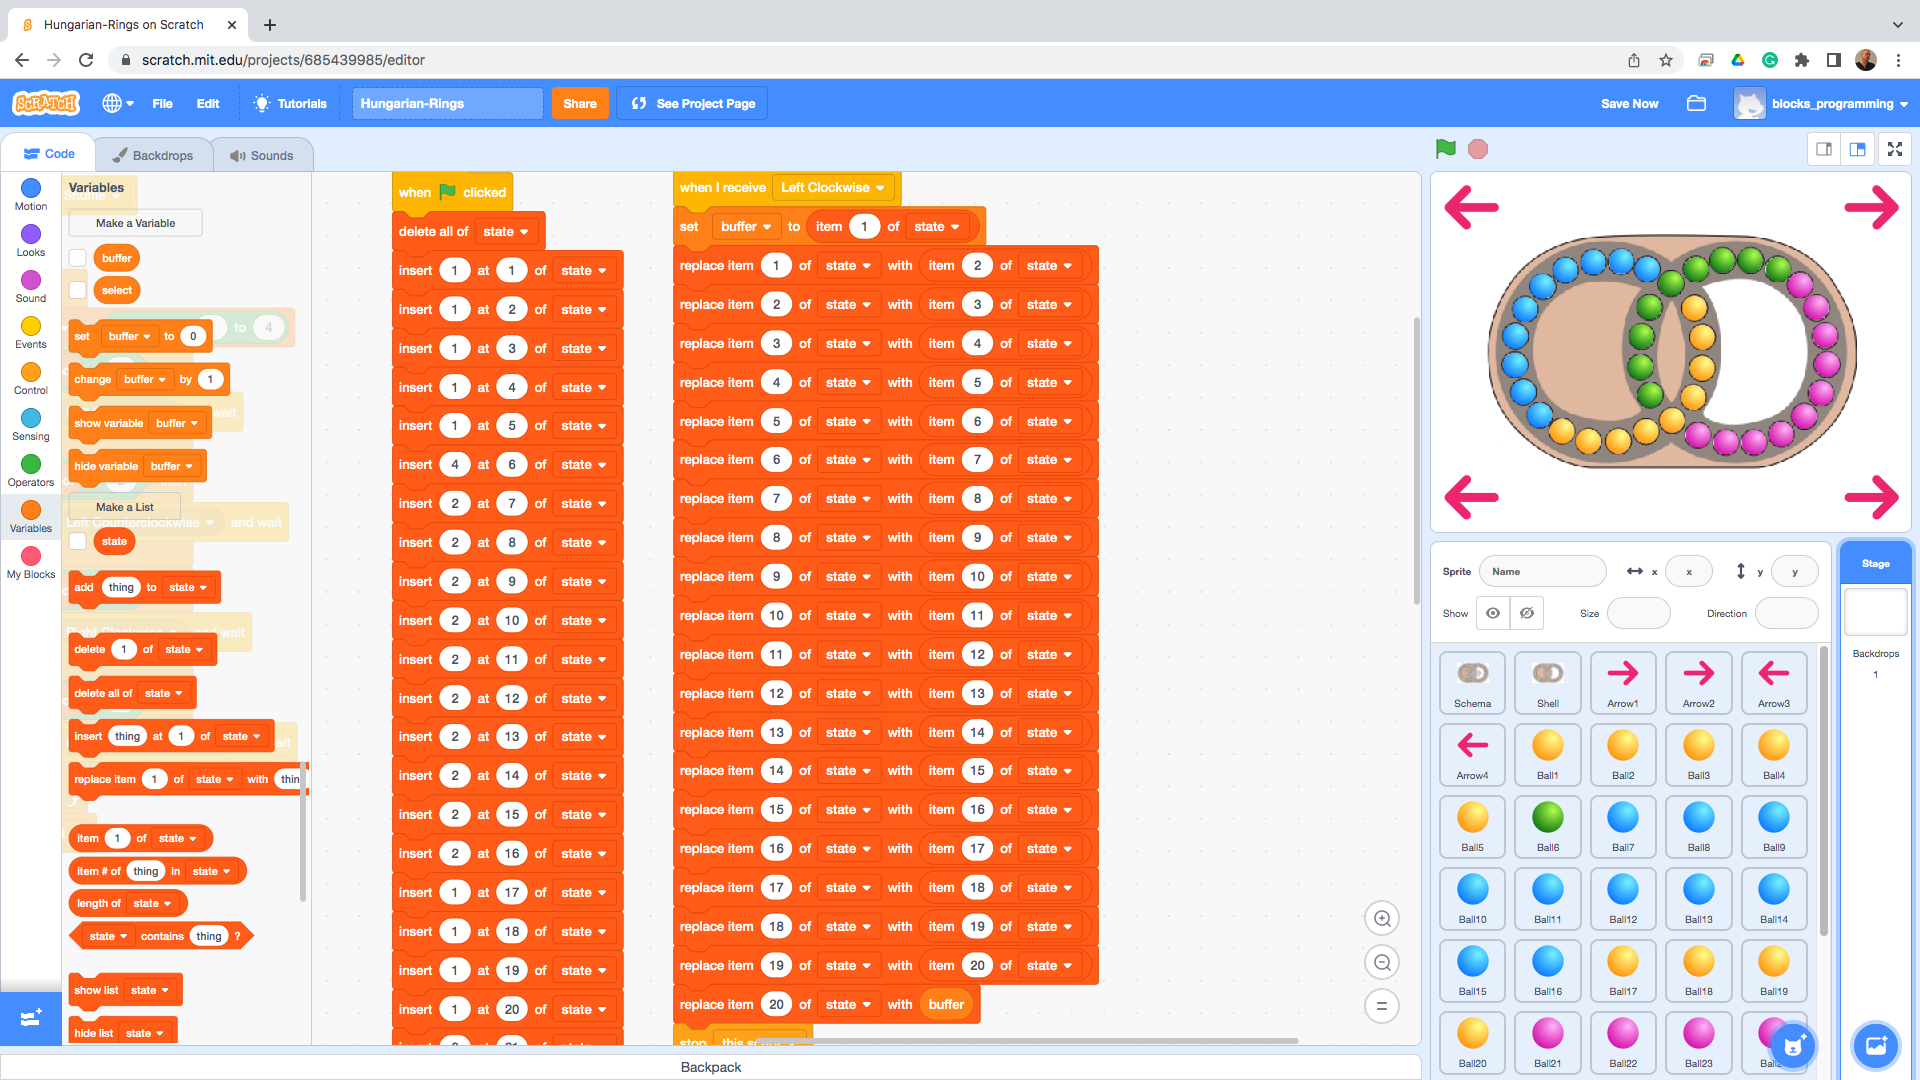
\includegraphics[width=1.0\linewidth,height=0.5\linewidth]{fig050028.png}
   \caption{Left ring clockwise rotation instructions}
\label{fig050028}
\end{figure}

The rotation of the left ring, counter-clockwise, is performed with the following sequence of actions (Fig. \ref{fig050029}).

\begin{figure}[H]
   \centering
   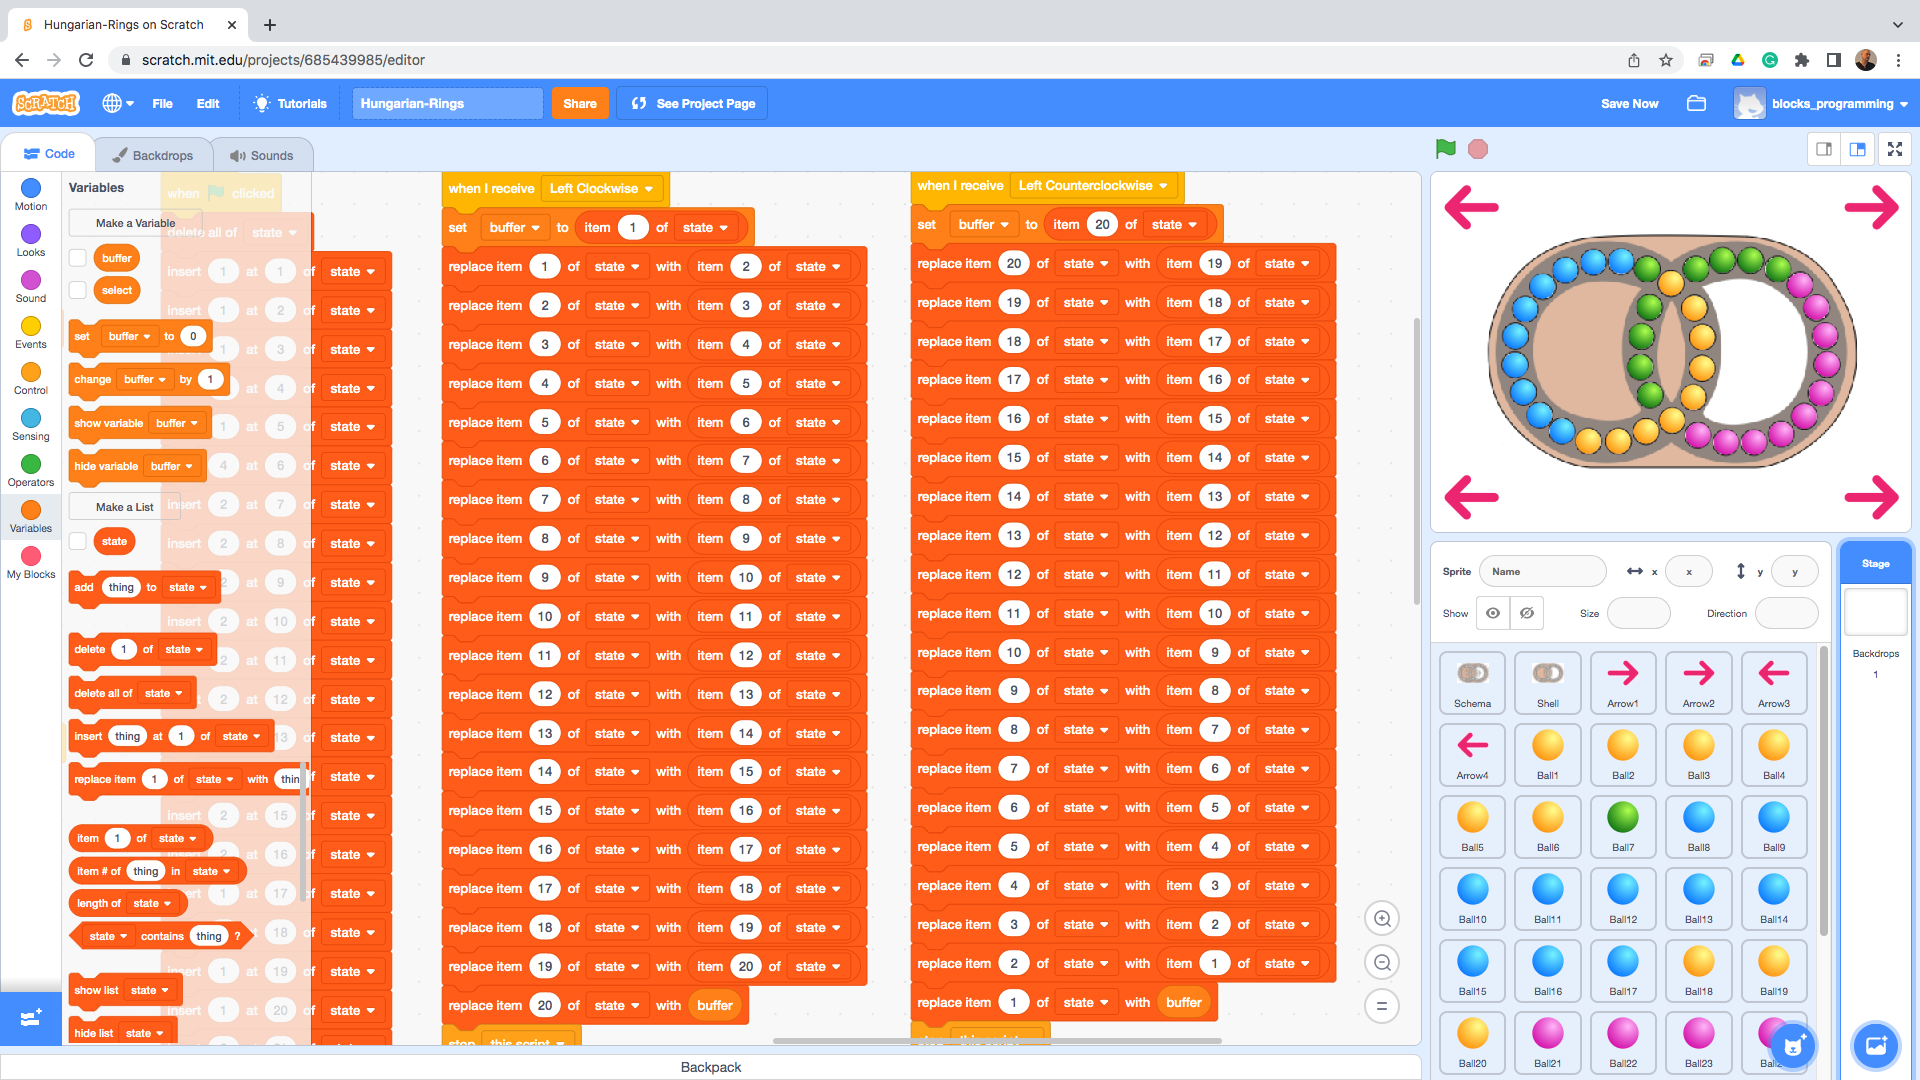
\includegraphics[width=1.0\linewidth,height=0.5\linewidth]{fig050029.png}
   \caption{Instructions for rotating the left ring counter-clockwise}
\label{fig050029}
\end{figure}

The rotation of the right ring, clockwise, is performed with the following sequence of actions (Fig. \ref{fig050030}).

\begin{figure}[H]
   \centering
   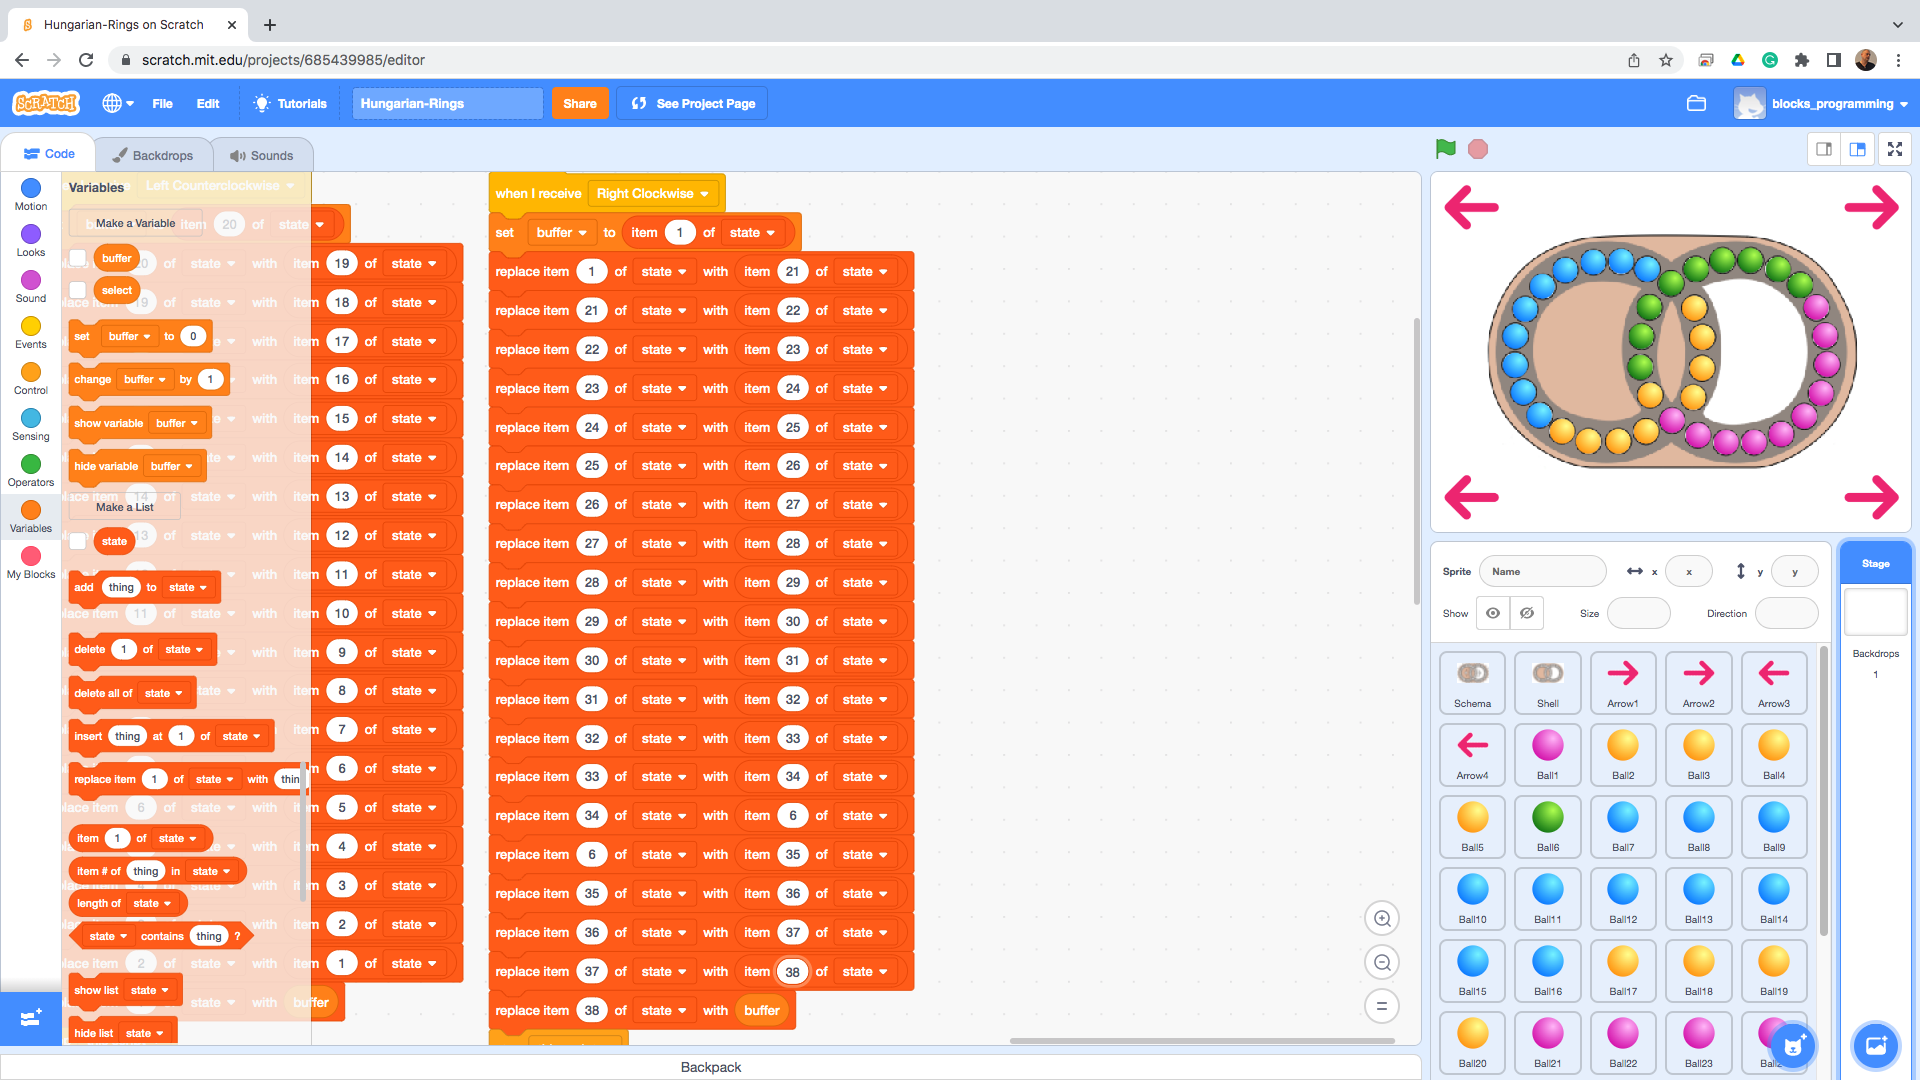
\includegraphics[width=1.0\linewidth,height=0.5\linewidth]{fig050030.png}
   \caption{Instructions for rotating the right ring clockwise}
\label{fig050030}
\end{figure}

The rotation of the right ring, counterclockwise, is performed with the following sequence of actions (Fig. \ref{fig050031}).

\begin{figure}[H]
   \centering
   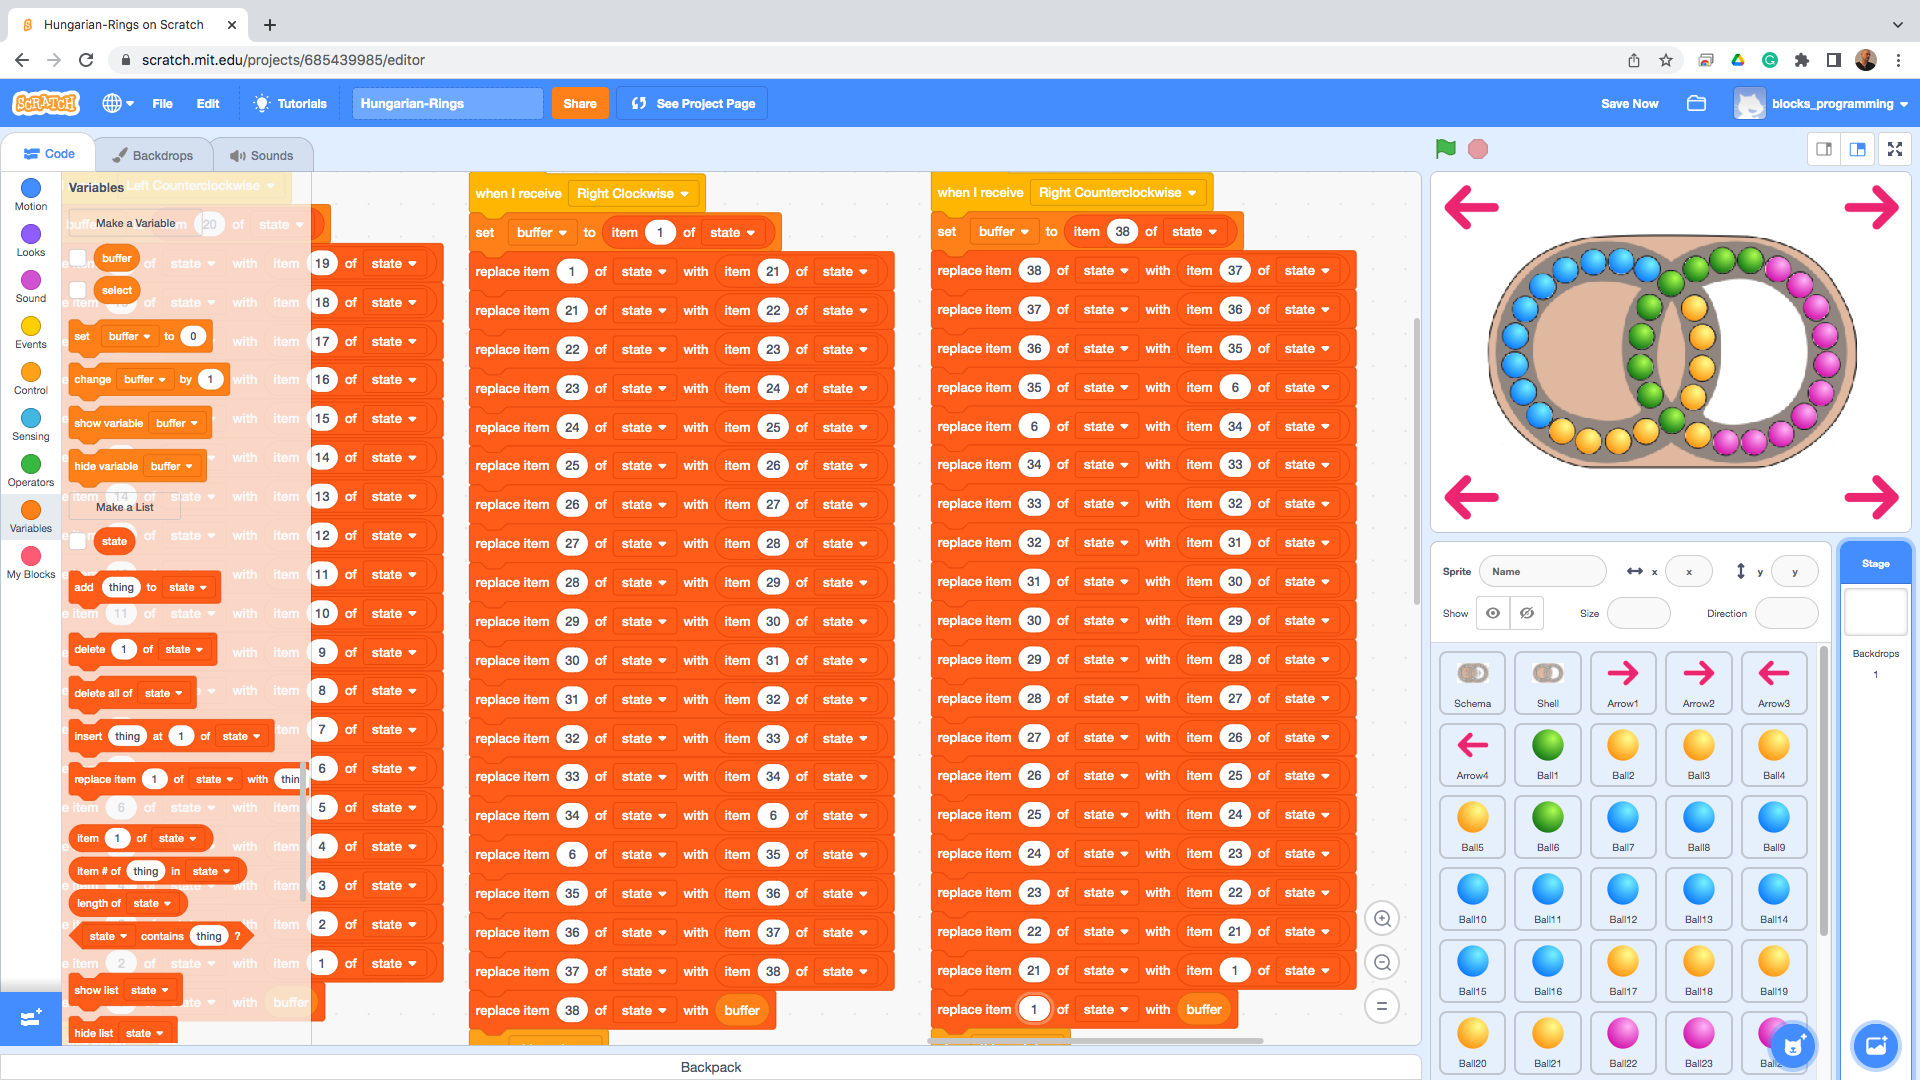
\includegraphics[width=1.0\linewidth,height=0.5\linewidth]{fig050031.png}
   \caption{Instructions for rotating the right ring counterclockwise}
\label{fig050031}
\end{figure}

\section{Publish the project}

After the execution of the last instructions, the game takes on its finished form. Of course, it is possible to continue development in the direction of ordering algorithms, but this task is far beyond the scope of the present exposition. Using the "SHARE" button, the game is published to the general audience (Fig. \ref{fig050032}).

\begin{figure}[H]
   \centering
   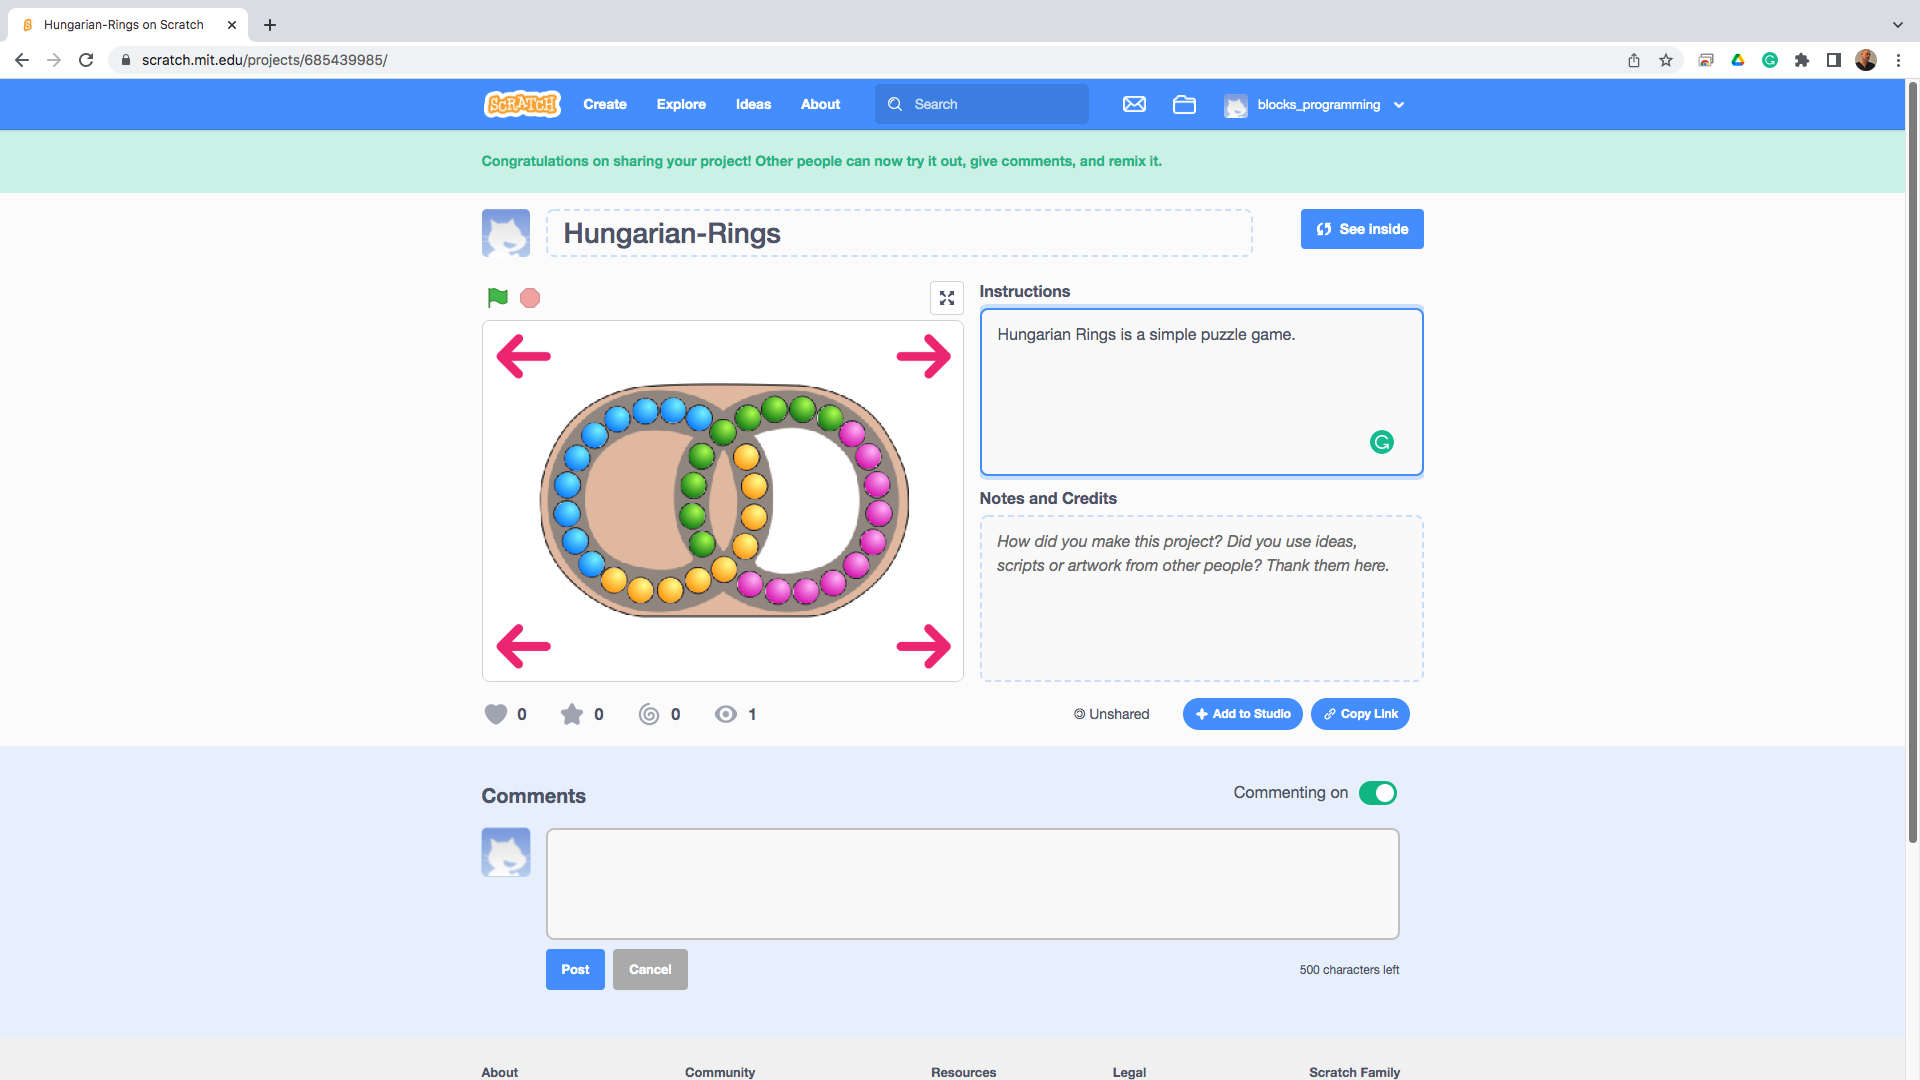
\includegraphics[width=1.0\linewidth,height=0.5\linewidth]{fig050032.png}
   \caption{Share the completed project}
\label{fig050032}
\end{figure}

The game has its finished look, but it must still be shaped as a final product. It would be nice to add functionality to arrange the puzzle. Help information needs to be included. It is possible to add counting time for stacking. All of the above brings additional complexity, which is beyond the scope of this presentation, but is an opportunity for extra exercise for the readers.
